\newgeometry{top=0.5cm}
\renewcommand{\chaptername}{Sección}
\chapter{Síntesis de un Circuito Dinámico}\label{ch:ch2label}
\section{Definición del circuito}
\subsection{Lógica CMOS Dinámica}
Este tipo de lógica pretende reducir el área de la lógica CMOS convencional (simplificando el layout en consecuencia) evitando las desventajas de una lógica estática tales como el consumo en estado estacionario o la degradación de niveles lógicos.
\newline Esto se consigue aprovechando el hecho de que existen muchas señales en un circuito que no es necesario estar generándolas durante todo el ciclo de reloj, es decir, que se mantengan válidas durante todo el mismo sino sólo en determinados momentos.
\newline El principio de operación se basa en sustituir los transistores pMOS del plano P por un único pMOS gobernado por un reloj y añadir un nMOS adicional gobernado por el mismo reloj. Al eliminar la red P casi en su totalidad, se nos permite reducir casi a la mitad el área ocupada con la bajada en la potencia de disipada que ello conlleva.
\newline Este tipo de circuitos se pueden resumir en el siguiente esquema \cite{TheoryImages}:
\begin{figure}[h]%[!ht]
\begin{center}
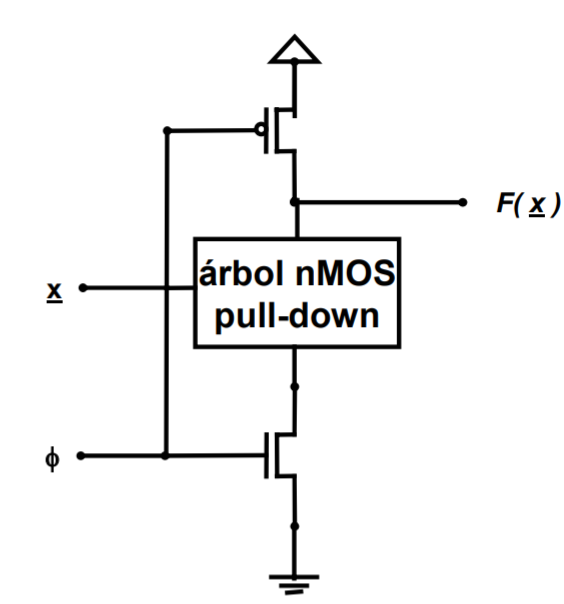
\includegraphics[width=0.5\textwidth]{figures/DynamicBasic.PNG}
\caption{Esquema general de un circuito CMOS de lógica dinámica}
\label{fig:DynBasic}
\end{center}
\end{figure}
\newline Donde \textit{X} serían las entradas de la puerta lógica y $\phi$ el reloj que gobierna los dos transistores comentados previamente.
\newgeometry{top=3cm, bottom=2cm}
\par Se tendrían dos fases diferenciadas:
\begin{enumerate}
    \item \textbf{Precarga:} El nodo de salida se carga a un valor lógico incondicionalmente mientras la red de evaluación permanece desconectada.
    \item \textbf{Evaluación:} La red de evaluación puede alterar el valor del nodo de salida.
\end{enumerate}
\begin{figure}[h]%[!ht]
\begin{center}
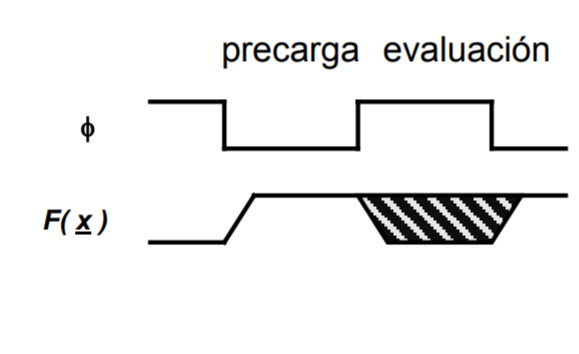
\includegraphics[width=0.4\textwidth]{figures/DynamicGraph.PNG}
\caption{Fases de un circuito CMOS dinámico}
\label{fig:Ib}
\end{center}
\end{figure}
\par \cite{TheoryExpl} En primer lugar, cuando el reloj ($\phi$) es cero, el nodo de salida de la puerta se lleva a nivel alto y será el transistor pMOS el que conducirá, lo que cargará en la salida un 1. Cuando $\phi$ se ponga a uno, en función de las entradas, la salida se quedará con el uno que tenía ya la capacidad asociada al nudo de salida no tiene sitio por donde descargarse ó el nMOS inferior se encargará de descargar la salida, dejando un cero. Además, hay que tener en cuenta que, durante la evaluación se pueden producir fugas de carga que descarguen el nodo a la salida.

\par Sin embargo, estos circuitos tienen problemas evidentes como su sensibilidad al ruido o el consumo asociado al reloj que puede llegar a ser muy elevado.
\subsection{Lógica Dominó}
Otro de los problemas de esta lógica es el encadenar etapas. El conflicto con este tipo de circuito radica en que puede ocurrir que una puerta sea algo más rápida que las anteriores y darle tiempo a evaluar mientras que las anteriores se encuentran todavía en fase de precarga. Para solucionar esto se emplea lo que se llama lógica dominó.
\begin{figure}[H]%[!ht]
\begin {center}
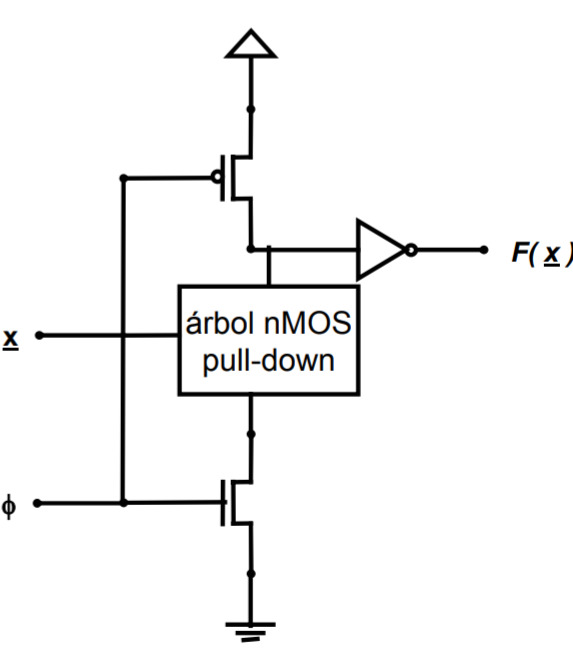
\includegraphics[width=0.4\textwidth]{figures/DominoBasic.PNG}
\caption{Esquemático básico de la Lógica Dominó}
\label{fig:Dominobasic}
\end {center}
\end{figure}
Como se puede observar, con la adición de un inversor CMOS a la salida, durante la fase de precarga se ataca a las siguientes etapas con ceros y aunque la evaluación de una puerta se atrase, ello sólo introduce un pequeño retraso en la evaluación definitiva pero no un error irreversible ya que la carga del nodo precargado no se puede disipar porque hasta que no se produzca la evaluación de las puertas anteriores, los transistores nMOS no conducen. (Esta es la razón por la que se le da el nombre de dominó, las primeras etapas determinan si las siguientes caen o no como piezas de dominó). 
\begin{figure}[h]%[!ht]
\begin {center}
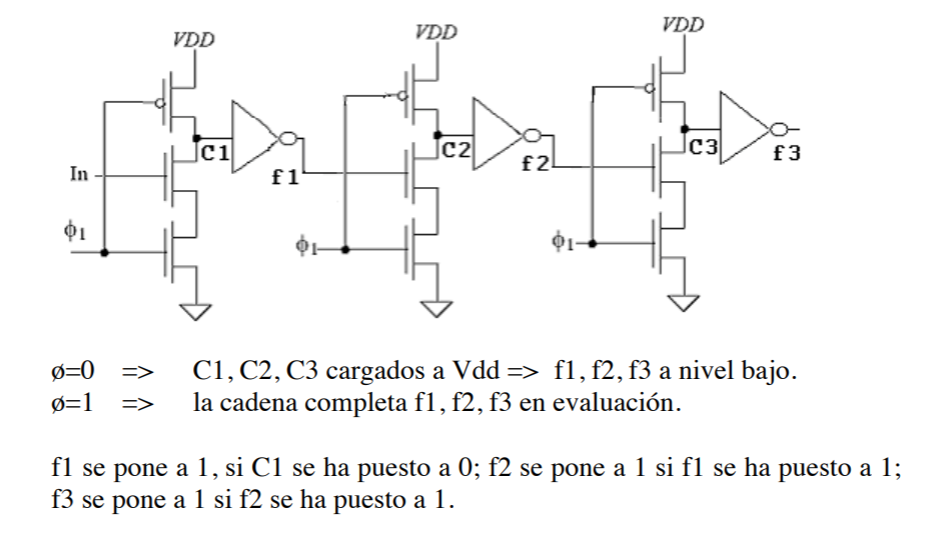
\includegraphics[width=1\textwidth]{figures/DominoEnc.PNG}
\caption{Encadenamiento de etapas con Lógica Dominó}
\label{fig:DominoEnc}
\end {center}
\end{figure} \newline
Con este esquema te aseguras de que todas las entradas son 0 durante la precarga lo que garantiza una única transición en las entradas (de 0 a 1) y reduce la capacidad del nodo de salida lo que facilita muy altas velocidades. \cite{TheoryAdvant}
\newline Sin embargo, estas puertas lógicas son únicamente no inversoras debido al inversor de la salida.
\subsection{Especificaciones}
Para esta práctica se dimensionarán los transistores con su longitud de canal mínima permitida por la tecnología AMS utilizada $0.35\mu m$ y su ancho de puerta mínimo $0.4\mu m$ para reducir las capacidades de entrada. La tensión de alimentación será la correspondiente a la tecnología MOS (3.3V).
\newline Para los transistores PMOS superior y nMOS inferior que controlarán la carga y descarga del nodo de salida, se emplearán $W_E = 1\mu m$ (nMOS) y $W_P =0.4\cdot W_E = 0.4\mu m$. La relación entre ambos anchos se mantendrá a lo largo de toda la práctica pero, en al final de esta sección se hará un análisis paramétrico de este parámetro. \newpage
\par Dicho esto, las cuestiones planteadas en el guion y que se irán respondiendo a lo largo de esta sección son las siguientes:
\begin{enumerate}
    \item ¿Qué Tipo de Lógica Dinámica es y qué Función Combinacional realiza?.
    \item ¿Qué porcentajes del Periodo de Reloj asignaría, en principio, a la Precarga y a la Evaluación?.
    \item Con los valores iniciales de WP y WE…. ¿Cuál es el valor máximo de la frecuencia Freq de Clock, supuesto el reloj simétrico, con tiempos fijos $t_{rise} = t_{fall} = 0.1 ns$?.
    \item Tomando $W_E$ como variable. ¿Cuál es su valor mínimo para operar a 500 MHz, con $t_{rise} = t_{fall} = 0.1 ns$?.
\end{enumerate}

\section{Captura del diseño}
Una vez se han dado las especificaciones necesarias, se ha procedido a crear una CellView nueva utilizando el programa Schematics L incluido en el Entorno de Cadence donde se ha creado el esquemático. Este ha sido el resultado:

\begin{figure}[h]%[!ht]
\begin {center}
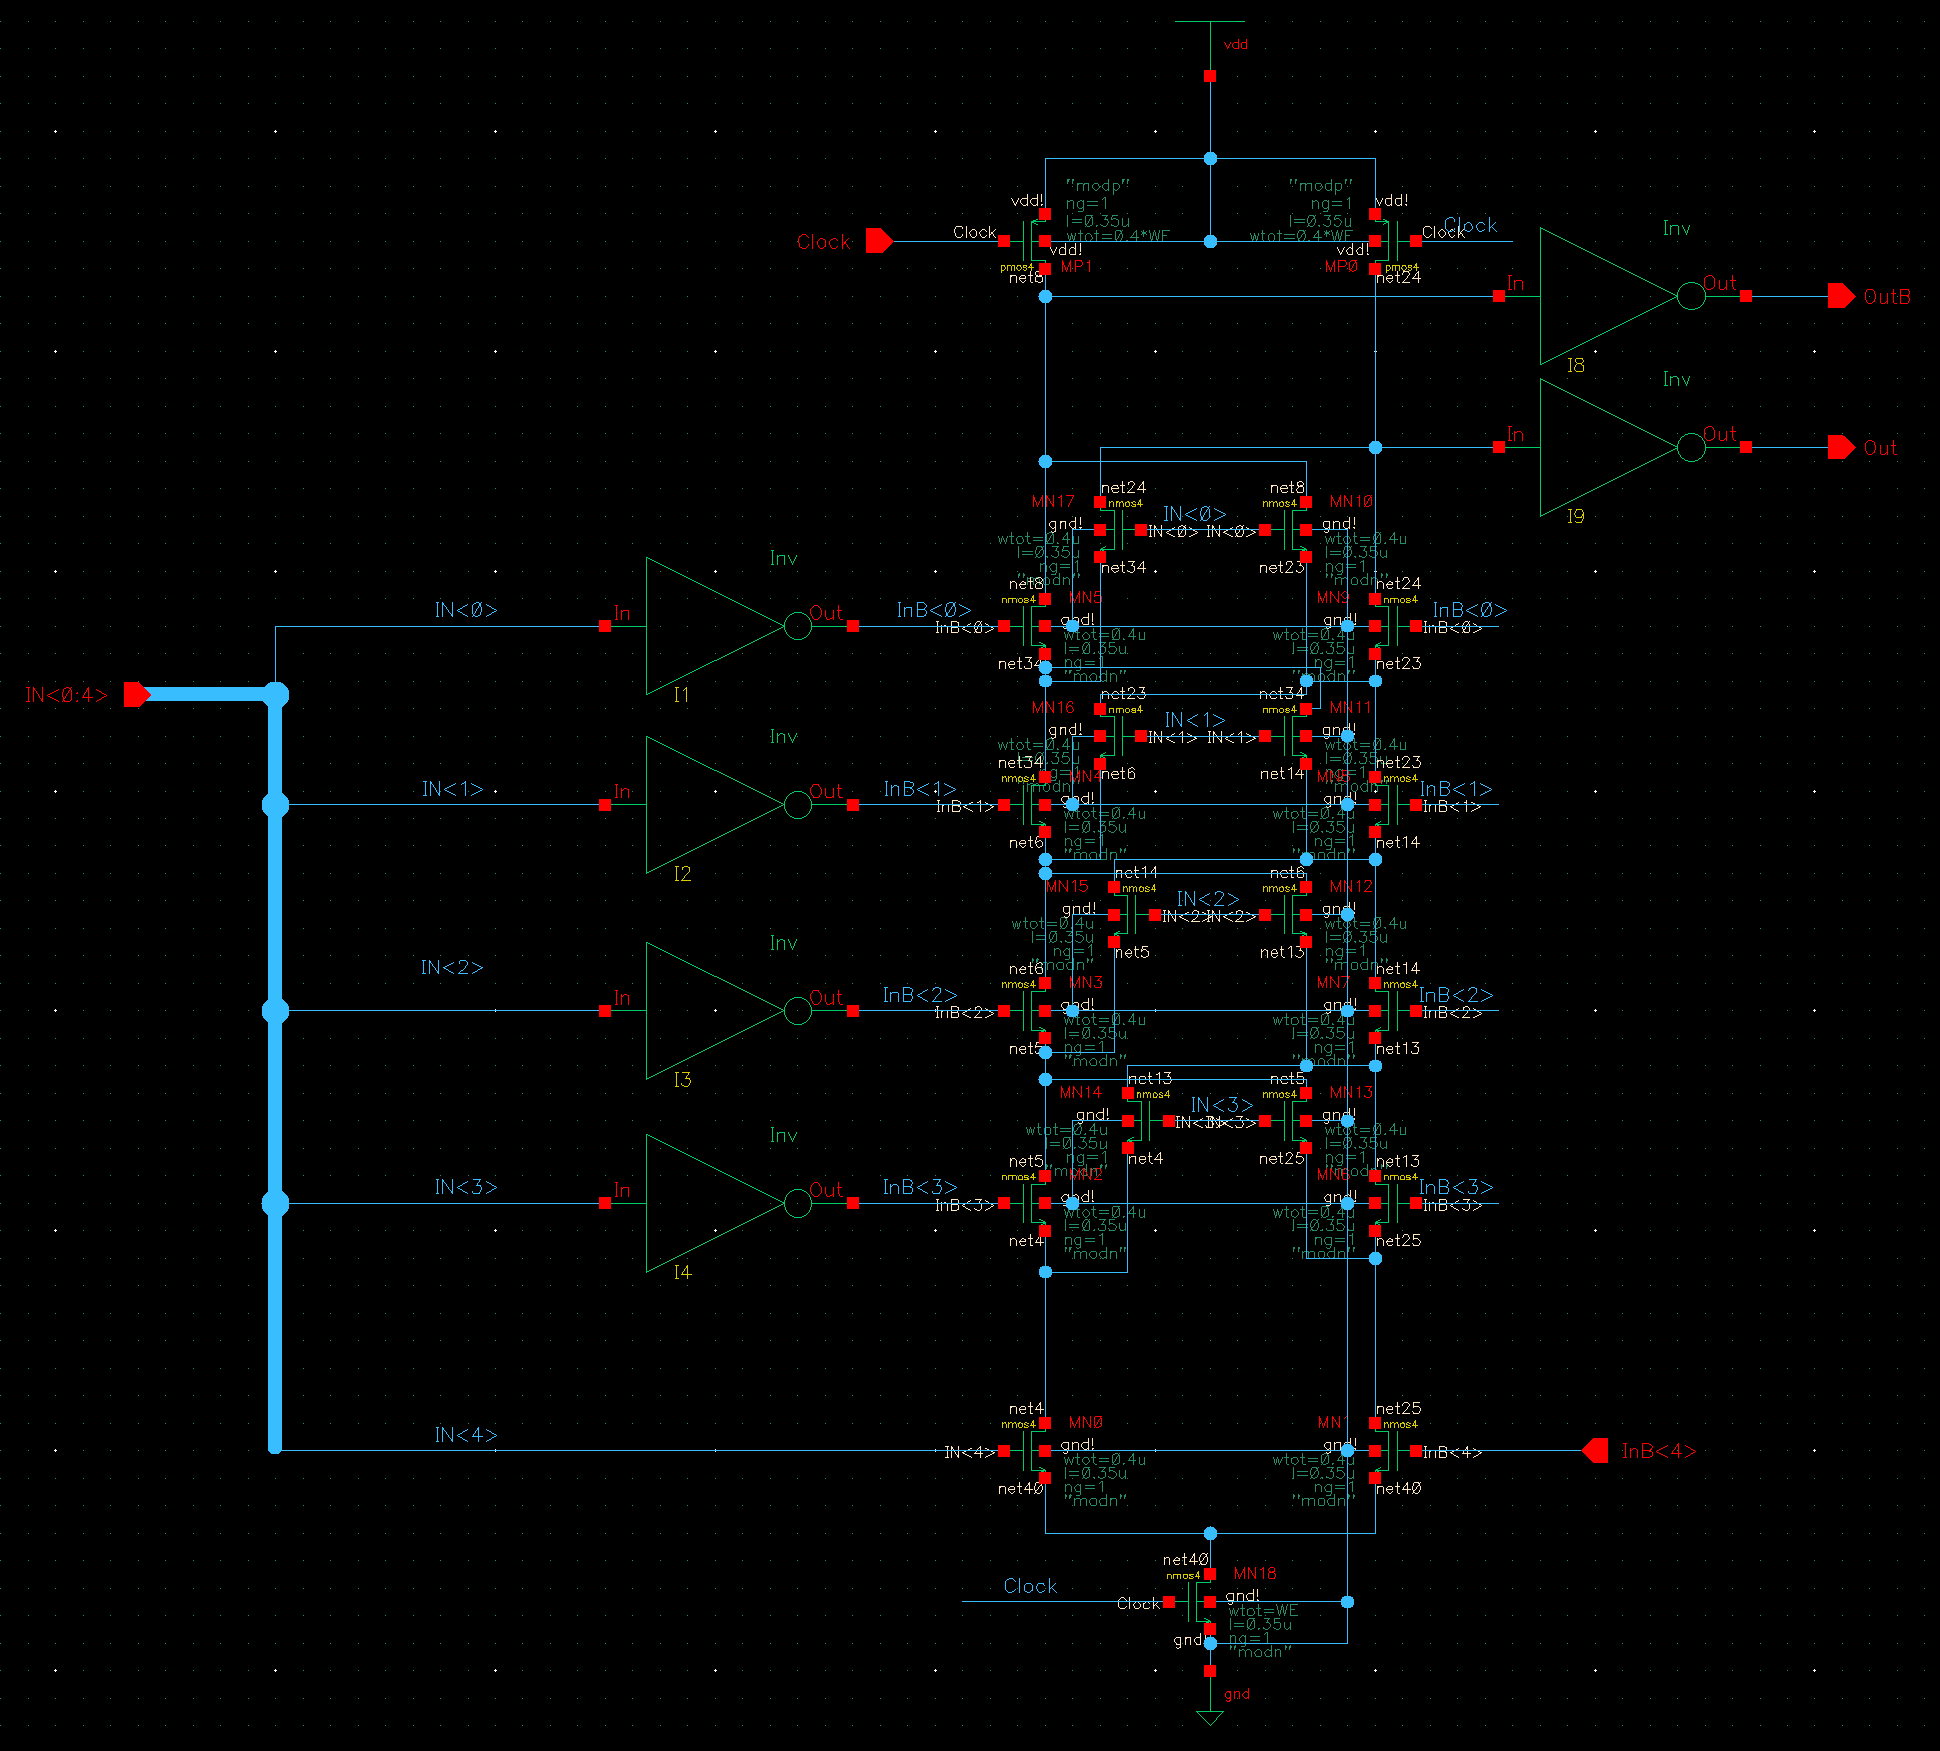
\includegraphics[width=1\textwidth]{figures/BlockDynSchem.PNG}
\caption{Esquema de la Etapa CMOS Dinámica (BlockDyn)}
\label{fig:BlockDynSchem}
\end {center}
\end{figure}
Se han utilizado los \textit{nmos4} y \textit{pmos4} de PRIMLIB, perteneciente a la tecnología \textbf{AMS TECH\_C35B4}. Además, se han utilizado las tomas de alimentación y de masa (vdd y gnd) pertenecientes a la librería analogLib, que es tecnoindependiente. \newline
Se ha introducido un parámetro, que esta vez no lo tomaremos como CDF sino que le daremos un valor en el ADE posteriormente para propósitos de simulación.
En cuanto a las dimensiones de los transistores, la longitud de canal es la mínima ($0.35\mu m$) y el ancho depende del tipo de MOS: como la movilidad de los electrones (portadores negativos) es 2.5 veces superior a la de los huecos (portadores positivos), el ancho del canal del NMOS se toma como el mínimo ($0.4\mu m$) y el ancho del PMOS es 2.5 veces mayor ($1\mu m$), como ya se ha comentado en las especificaciones.
\par Como el esquemático tiene tantos transistores, se ha decidido tomar la idea que aparece en el guion de incluir capturas de pantalla con un zoom sobre determinadas partes del esquemático:
\begin{figure}[h]%[!ht]
\begin{center}
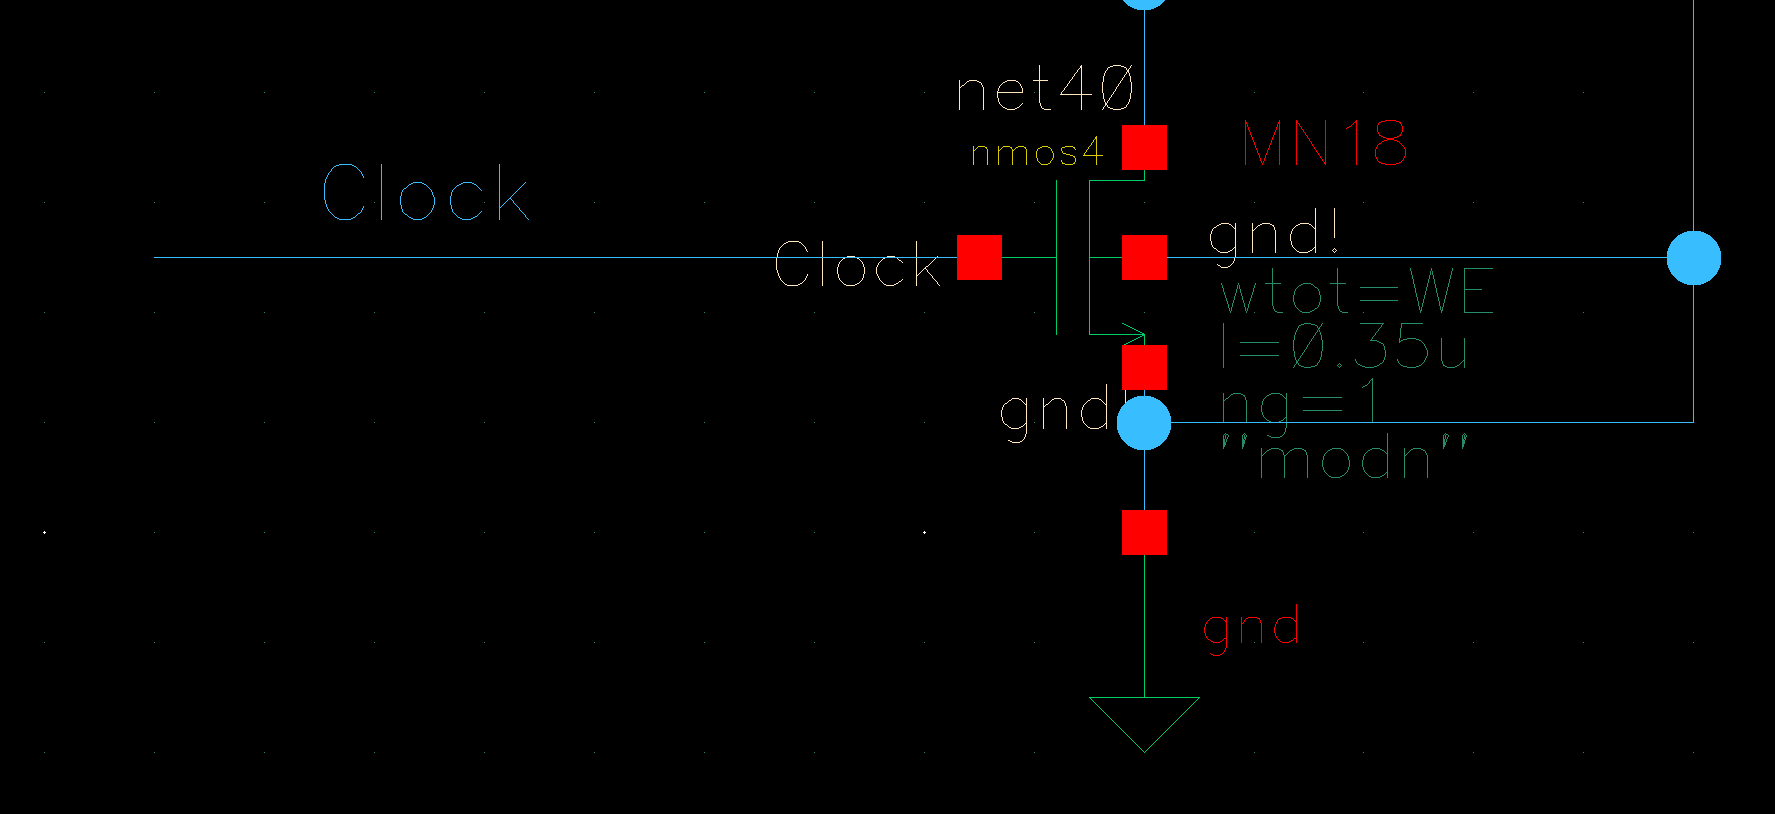
\includegraphics[width=0.8\textwidth]{figures/DeatilNMOS.PNG}
\label{fig:CDF}
\end{center}
\end{figure}
\begin{figure}[h]%[!ht]
\begin{center}
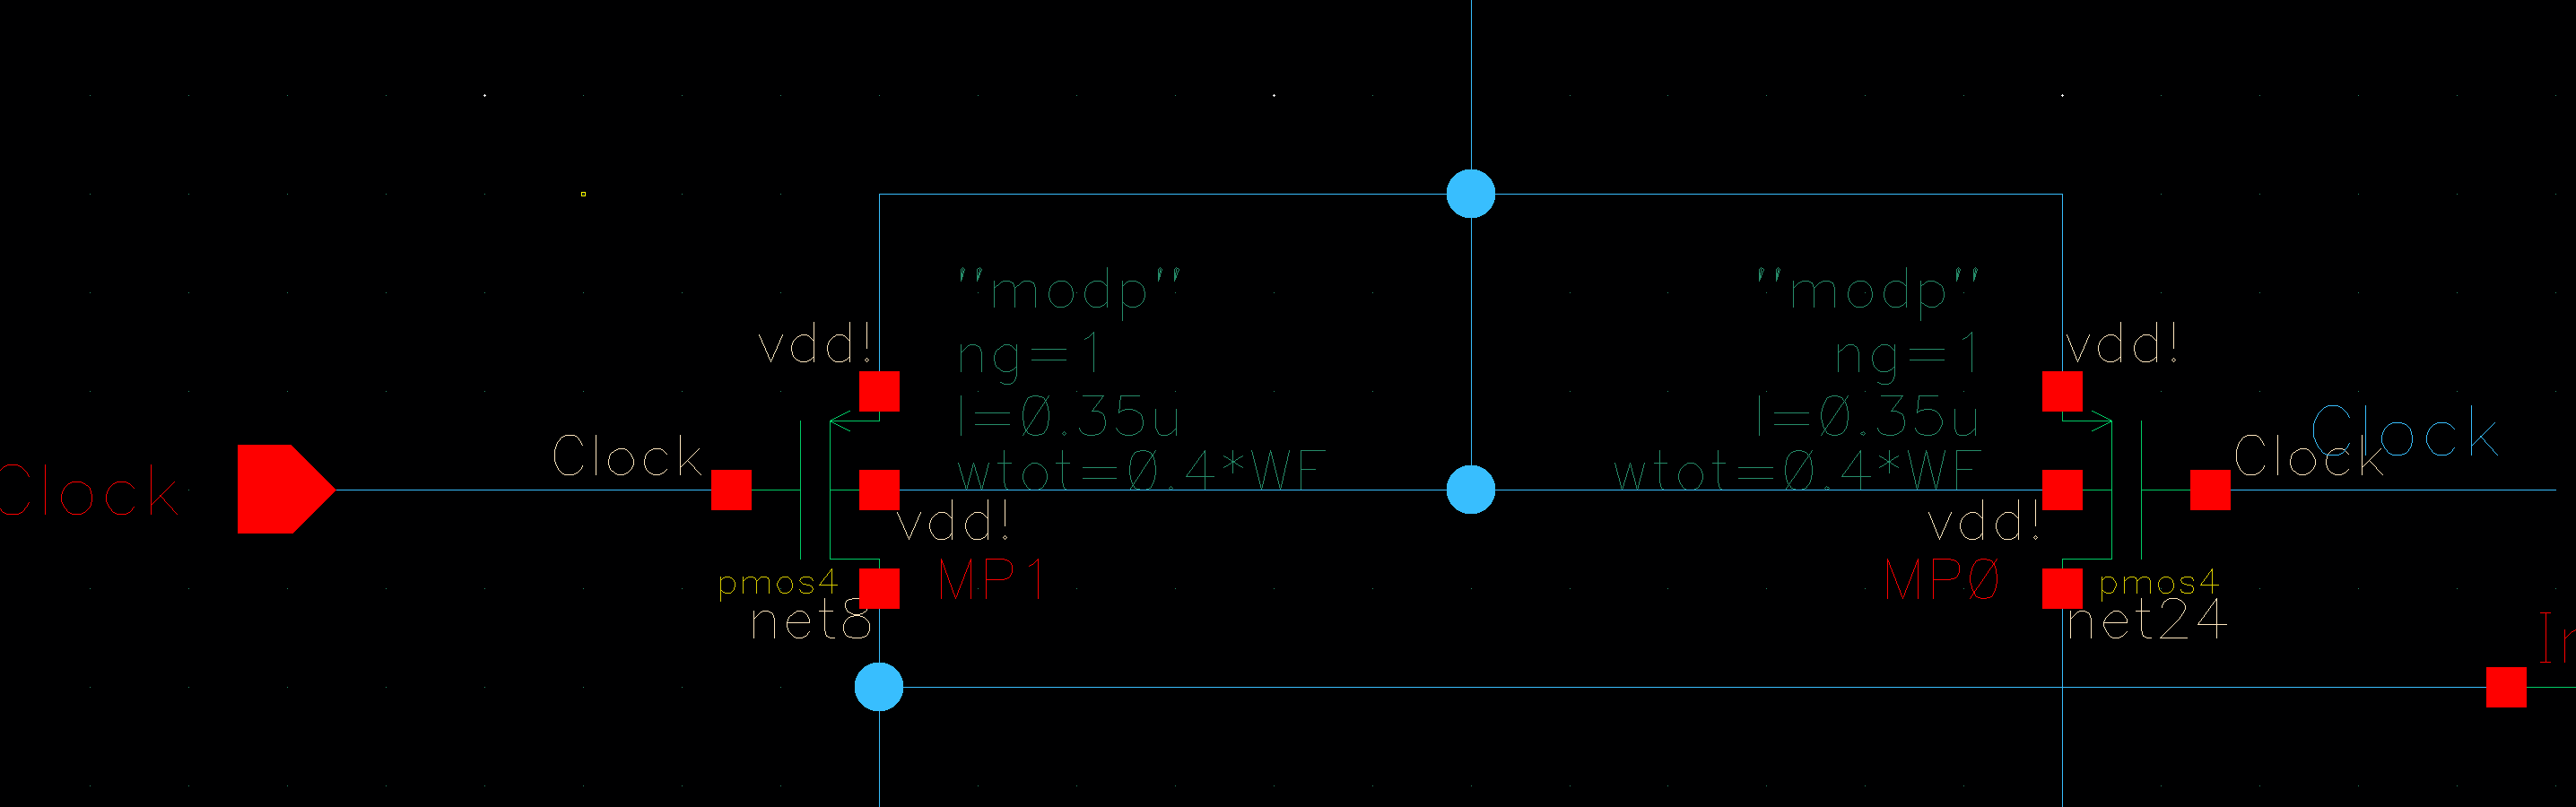
\includegraphics[width=0.8\textwidth]{figures/DetailPMOS.PNG}
\caption{Vista en detalle del pMOS de precarga y el NMOS de descarga de la red que ejecuta la función lógica}
\end{center}
\end{figure} \newline
En este esquemático se ha utilizado otra herramienta del Schematic Editor L de Cadence que serían los buses, que nos permiten hacer cables de varios bits de ancho a diferencia de Wire (Narrow) que sólo podía transportar un bit. Gracias a la conexión por nombre se han etiquetado los distintos bits que salían del bus y se han conectado \say{by name} a las puertas de la escalera central del esquemático. Los inversores utilizados pertenecen a la librería PIEZAS\_DIG, son en concreto la célula \textbf{Inv}.
\newline Si observamos la estructura del esquemático, el tipo de lógica dinámica que realiza es \textbf{dominó}, sólo hay que comparar el esquemático con la figura \ref{fig:Dominobasic} para darnos cuenta de que, aparte de cumplir con las características de un Circuito CMOS dinámico, presenta inversores en sus salidas. Además, hay un pMOS extra que precarga los nudos internos para solucionar el charge sharing.
\section{Simulaciones}
El resto de cuestiones quedarán respondidas tras haber realizado una simulación que dividiremos en tres etapas 
\subsection{Análisis transitorio inicial}
Se ha construido el testbench propuesto en el guion de la práctica:
\begin{figure}[h]%[!ht]
\begin{flushleft}
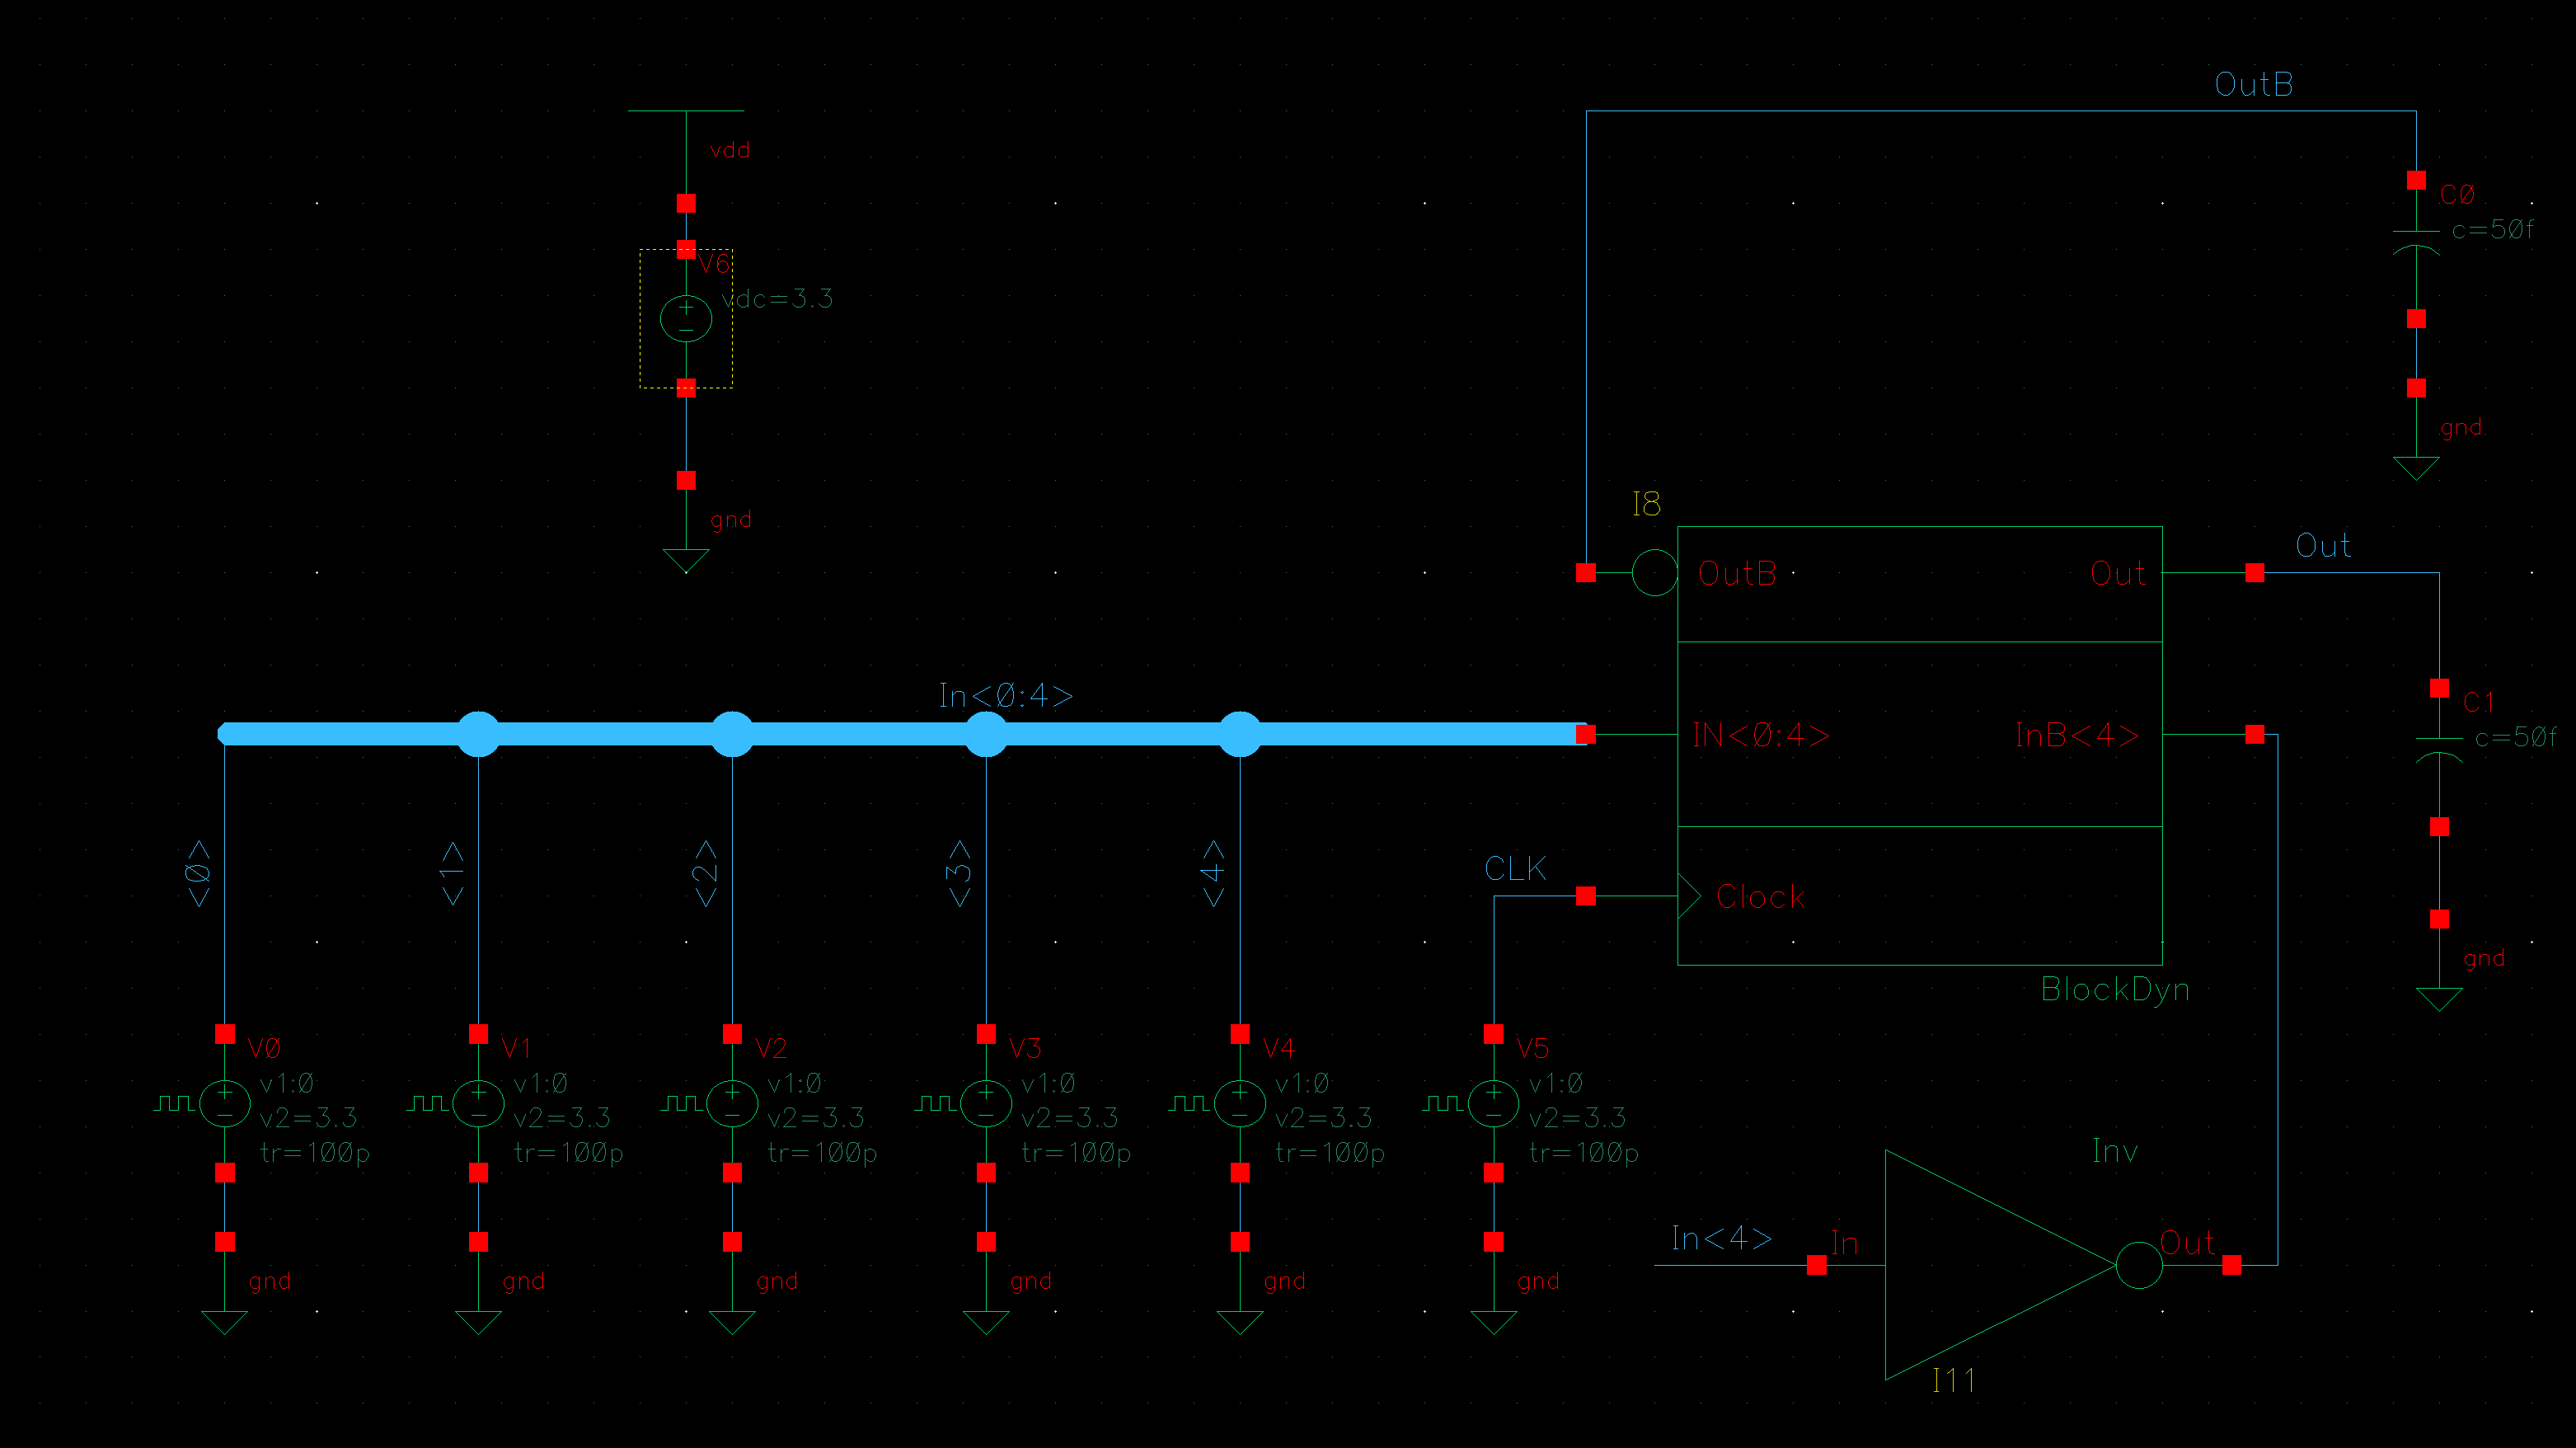
\includegraphics[width=1.1\textwidth]{figures/BlockDynTBSchem.PNG}
\caption{Banco de pruebas para BlockDyn}
\label{fig:BlockDynTBSchem}
\end{flushleft}
\end{figure} \newline
Donde se ha estimulado el circuito con un reloj de periodo \textit{TPeriod} parametrizable y simétrico y se han ido colocando señales cuadradas a cada entrada de forma que se reproduzcan todas las combinaciones posibles de entradas. 
\newpage Aquí se muestran como ejemplos In<1>, In<2>  e In<5>, de izquierda a derecha:
\begin{figure*}[h]
\begin{multicols}{3}
    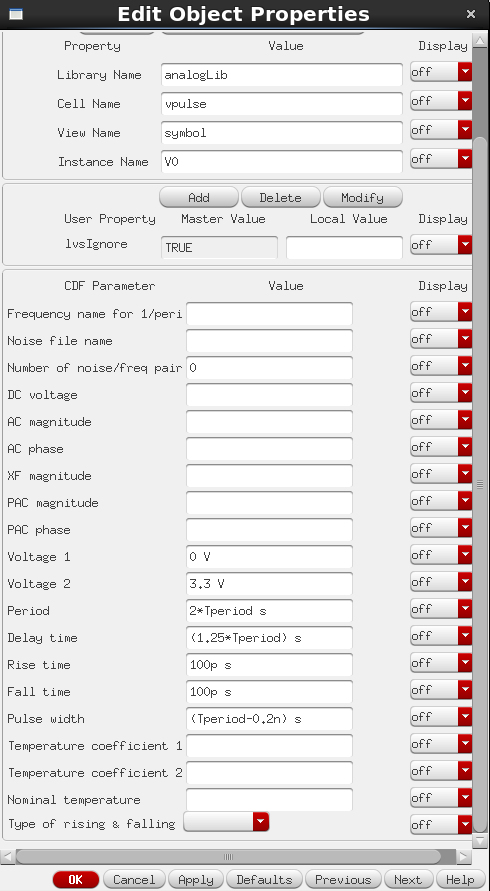
\includegraphics[width=1\linewidth]{figures/In1Config.PNG}\par 
    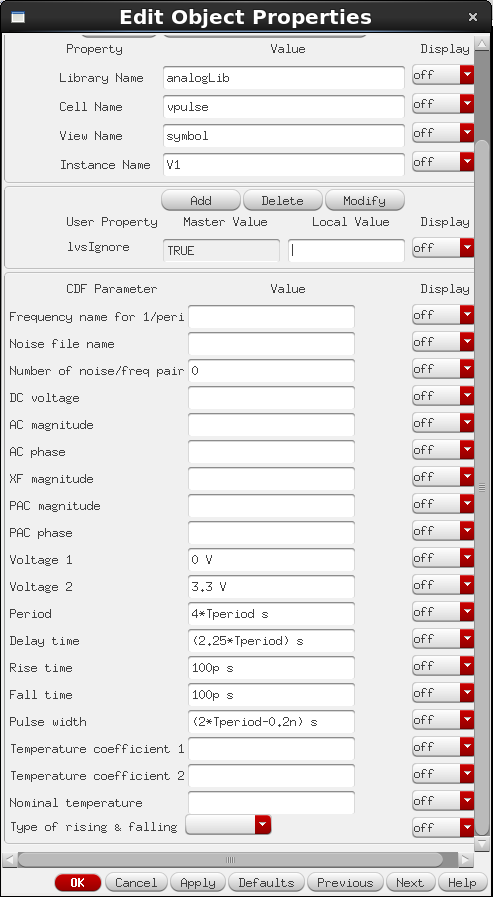
\includegraphics[width=1\linewidth]{figures/In2Config.PNG}\par
    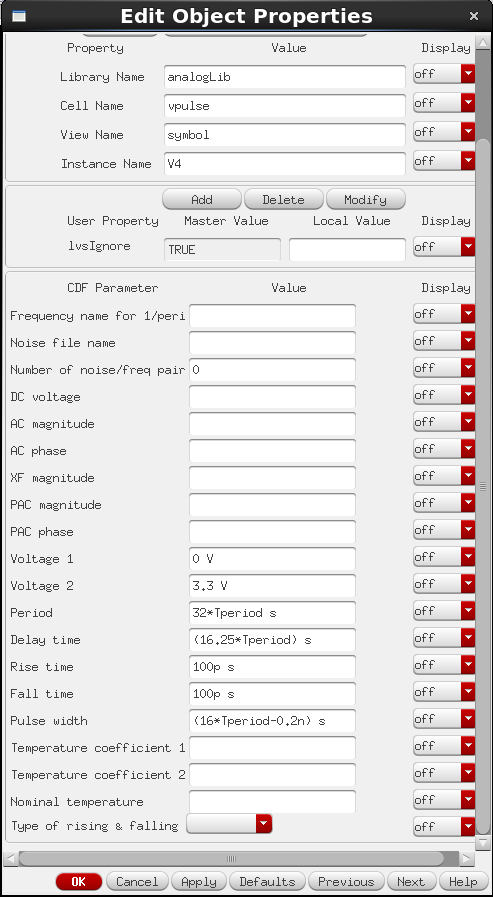
\includegraphics[width=1\linewidth]{figures/In4Config.PNG}\par 
    \end{multicols}
    \caption{Señales de entrada}
\end{figure*} \newline
Con este testbench, se ha abierto el Analog Design Environment L y se ha configurado el siguiente estado denominado \textit{state1}:
\begin{figure}[H]%[!ht]
\begin {center}
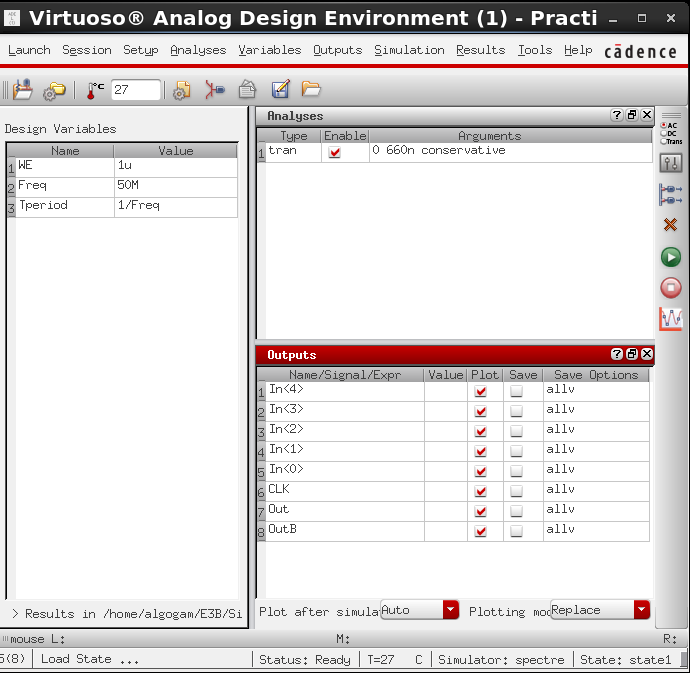
\includegraphics[width=0.6\textwidth]{figures/State1Config.PNG}
\caption{Estado con los valores iniciales de la simulación}
\label{fig:State1}
\end {center}
\end{figure} 

Donde se ha puesto, tal y como se propone en las especificaciones de la práctica se ha comenzado con una frecuencia de 50MHz y un ancho para los transistores de tipo N $1\mu m$.
\newpage Tras ejecutar la simulación, se obtuvo el siguiente resultado:
\begin{figure}[h]%[!ht]
\begin {center}
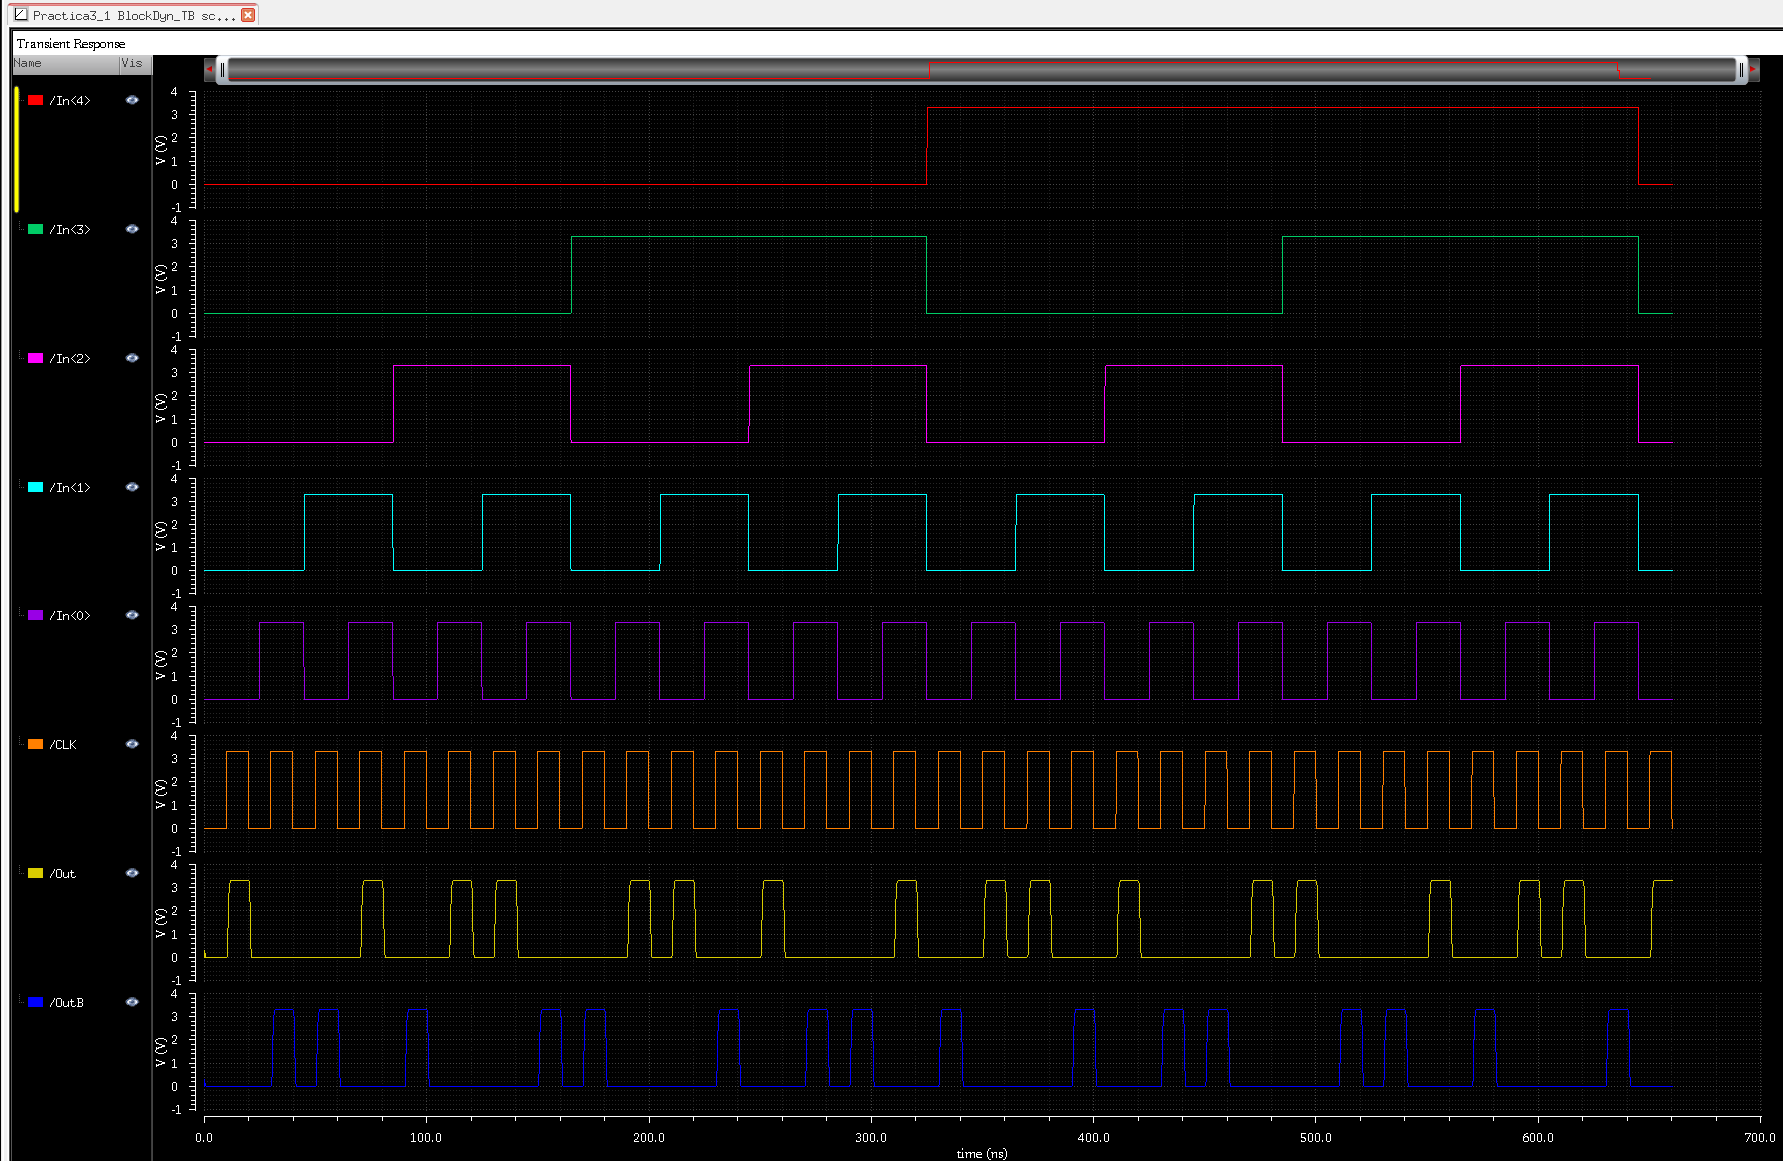
\includegraphics[width=1\textwidth]{figures/GraphState1TB.PNG}
\caption{Gráfica con los resultados de la simulación inicial}
\label{fig:GraphState1}
\end {center}
\end{figure} \newline
Si observamos atentamente las dos salidas vemos que OutB es la negada de Out pero sólamente cuando el reloj (traza naranja) vale 1. ¿Qué significa esto? Bien, esto es lógica CMOS dinámica, cuando el reloj está a cero, nos encontramos en la fase de precarga y al ser lógica dominó con un inversor a la salida, esta vale 0 en vez de 1 en la fase de precarga siempre, tanto para Out como OutB. En la fase de evaluación, si nos fijamos en las entradas vemos que sólamente cuando un número impar de ellas están a nivel alto, Out devuelve un 1 y, al contrario, cuando el número de unos es par, es OutB devuelve un 1, es decir, estamos ante un detector de paridad en la que Out es la señal de paridad Par y OutB la de paridad Impar.
\par En esta simulación se ha decidido poner el reloj simétrico pero no tiene por qué ser así ya que invertir la mitad de tiempo en la precarga cuando a lo mejor, por los tiempos de propagación, no es necesario darle todo ese tiempo para que el nudo de salida se ponga a uno.  Por lo tanto, sería mejor un mayor porcentaje del reloj a uno que a cero eso sí, teniendo en cuenta el retardo $t_{pmin}$ denotado en la figura 1 del guion \cite{Guion} y que, si dejamos demasiado tiempo el reloj a uno se pueden producir fugas demasiado grandes que degradarán el nivel de la señal de salida.  De la misma forma se debe respetar $t_{Emin}$ para que al circuito le dé tiempo a evaluar correctamente las entradas\newpage
\subsection{Análisis paramétrico con la frecuencia}
El siguiente paso es realizar un análisis en frecuencia con el valor de $W_E$ fijo para hallar cuál es la frecuencia máxima de operación a la cual este circuito sigue funcionando:
\begin{figure}[H]%[!ht]
\begin {center}
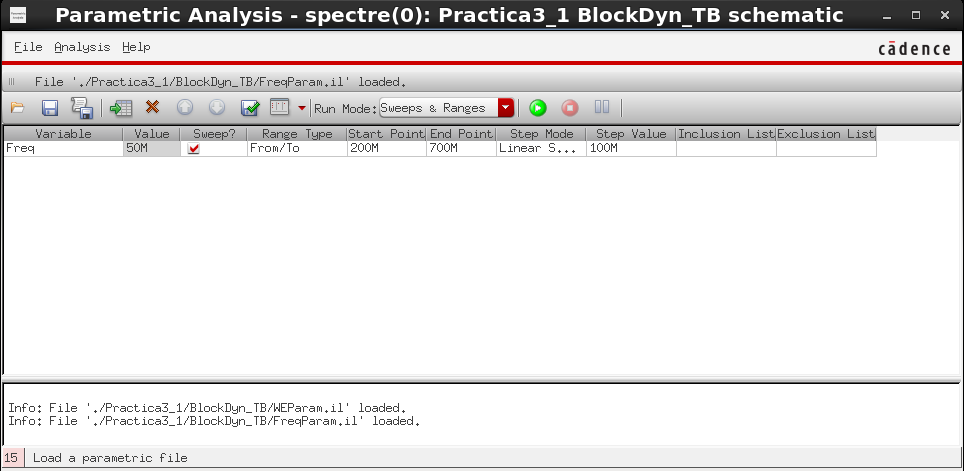
\includegraphics[width=1\textwidth]{figures/FreqParamConfig.PNG}
\caption{Configuración del análisis paramétrico en frecuencia}
\label{fig:ConfigFreqParam}
\end {center}
\end{figure} 
Además, se ha definido el siguiente estado, donde sólo se mostrarán las salidas y, además, se ha reducido el tiempo de simulación ya que las frecuencias altas tardan mucho en simular y las señales de salida son tan estrechas que no merecía la pena estar simulando durante tanto rato:
\begin{figure}[H]%[!ht]
\begin {center}
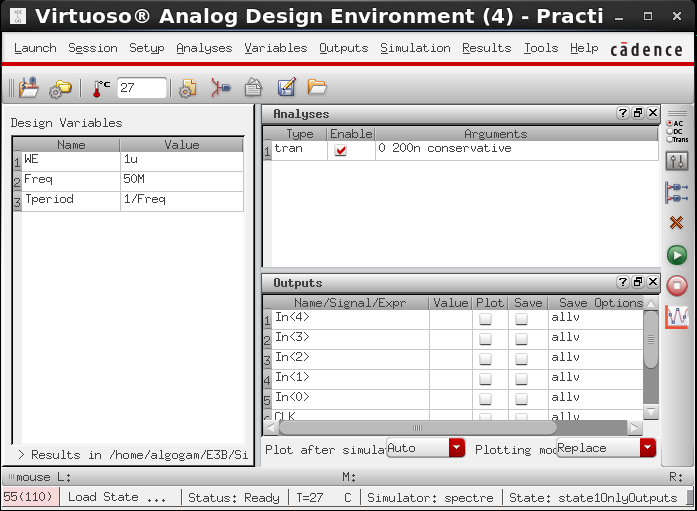
\includegraphics[width=0.85\textwidth]{figures/State1OnlyOutputsConfig.PNG}
\caption{Estado 1 con sólo las entradas}
\label{fig:ConfigState1OnlyOutputs}
\end {center}
\end{figure} 
Cabe destacar que se hicieron dos \say{Run} de la simulación, una desde 200MHz hasta 700MHz y otra desde 700MHz hasta 1.2GHz, algo excesivo pero con la intención de ver la evolución de la salida:
\begin{figure}[H]%[!ht]
\begin {center}
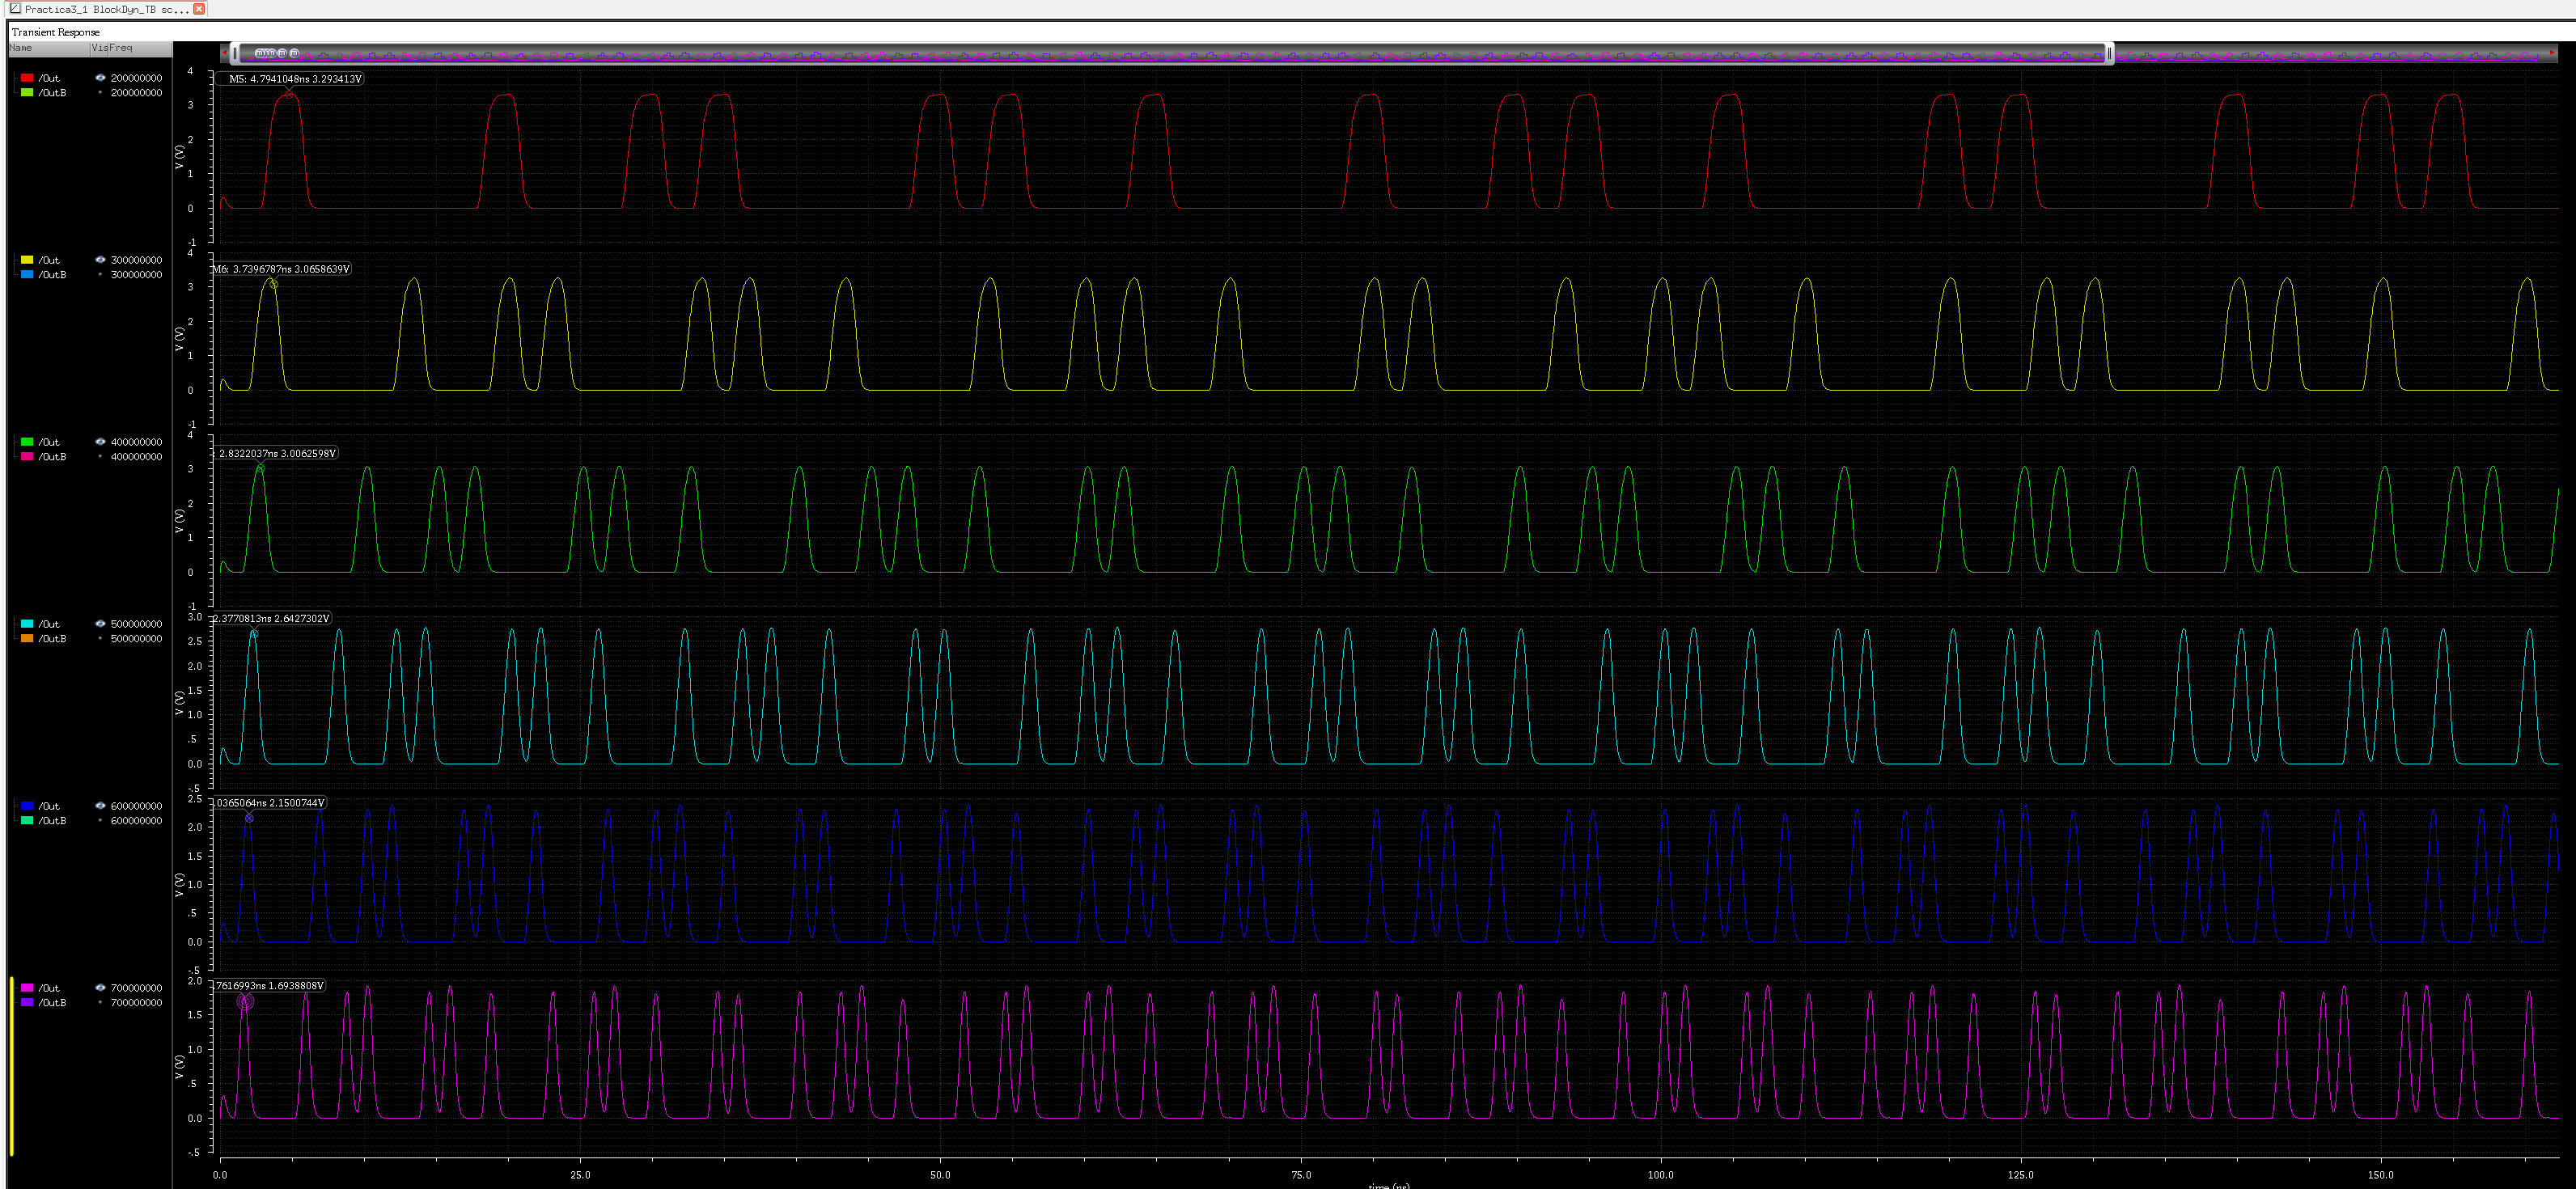
\includegraphics[width=1.1\textwidth]{figures/ParamFreqGraphNOVALIDO.PNG}
\caption{Gráfica del análisis paramétrico 200-700MHz}
\label{fig:GraphFreq1}
\end {center}
\end{figure} 
\vspace{-1cm}
\begin{figure}[H]%[!ht]
\begin {center}
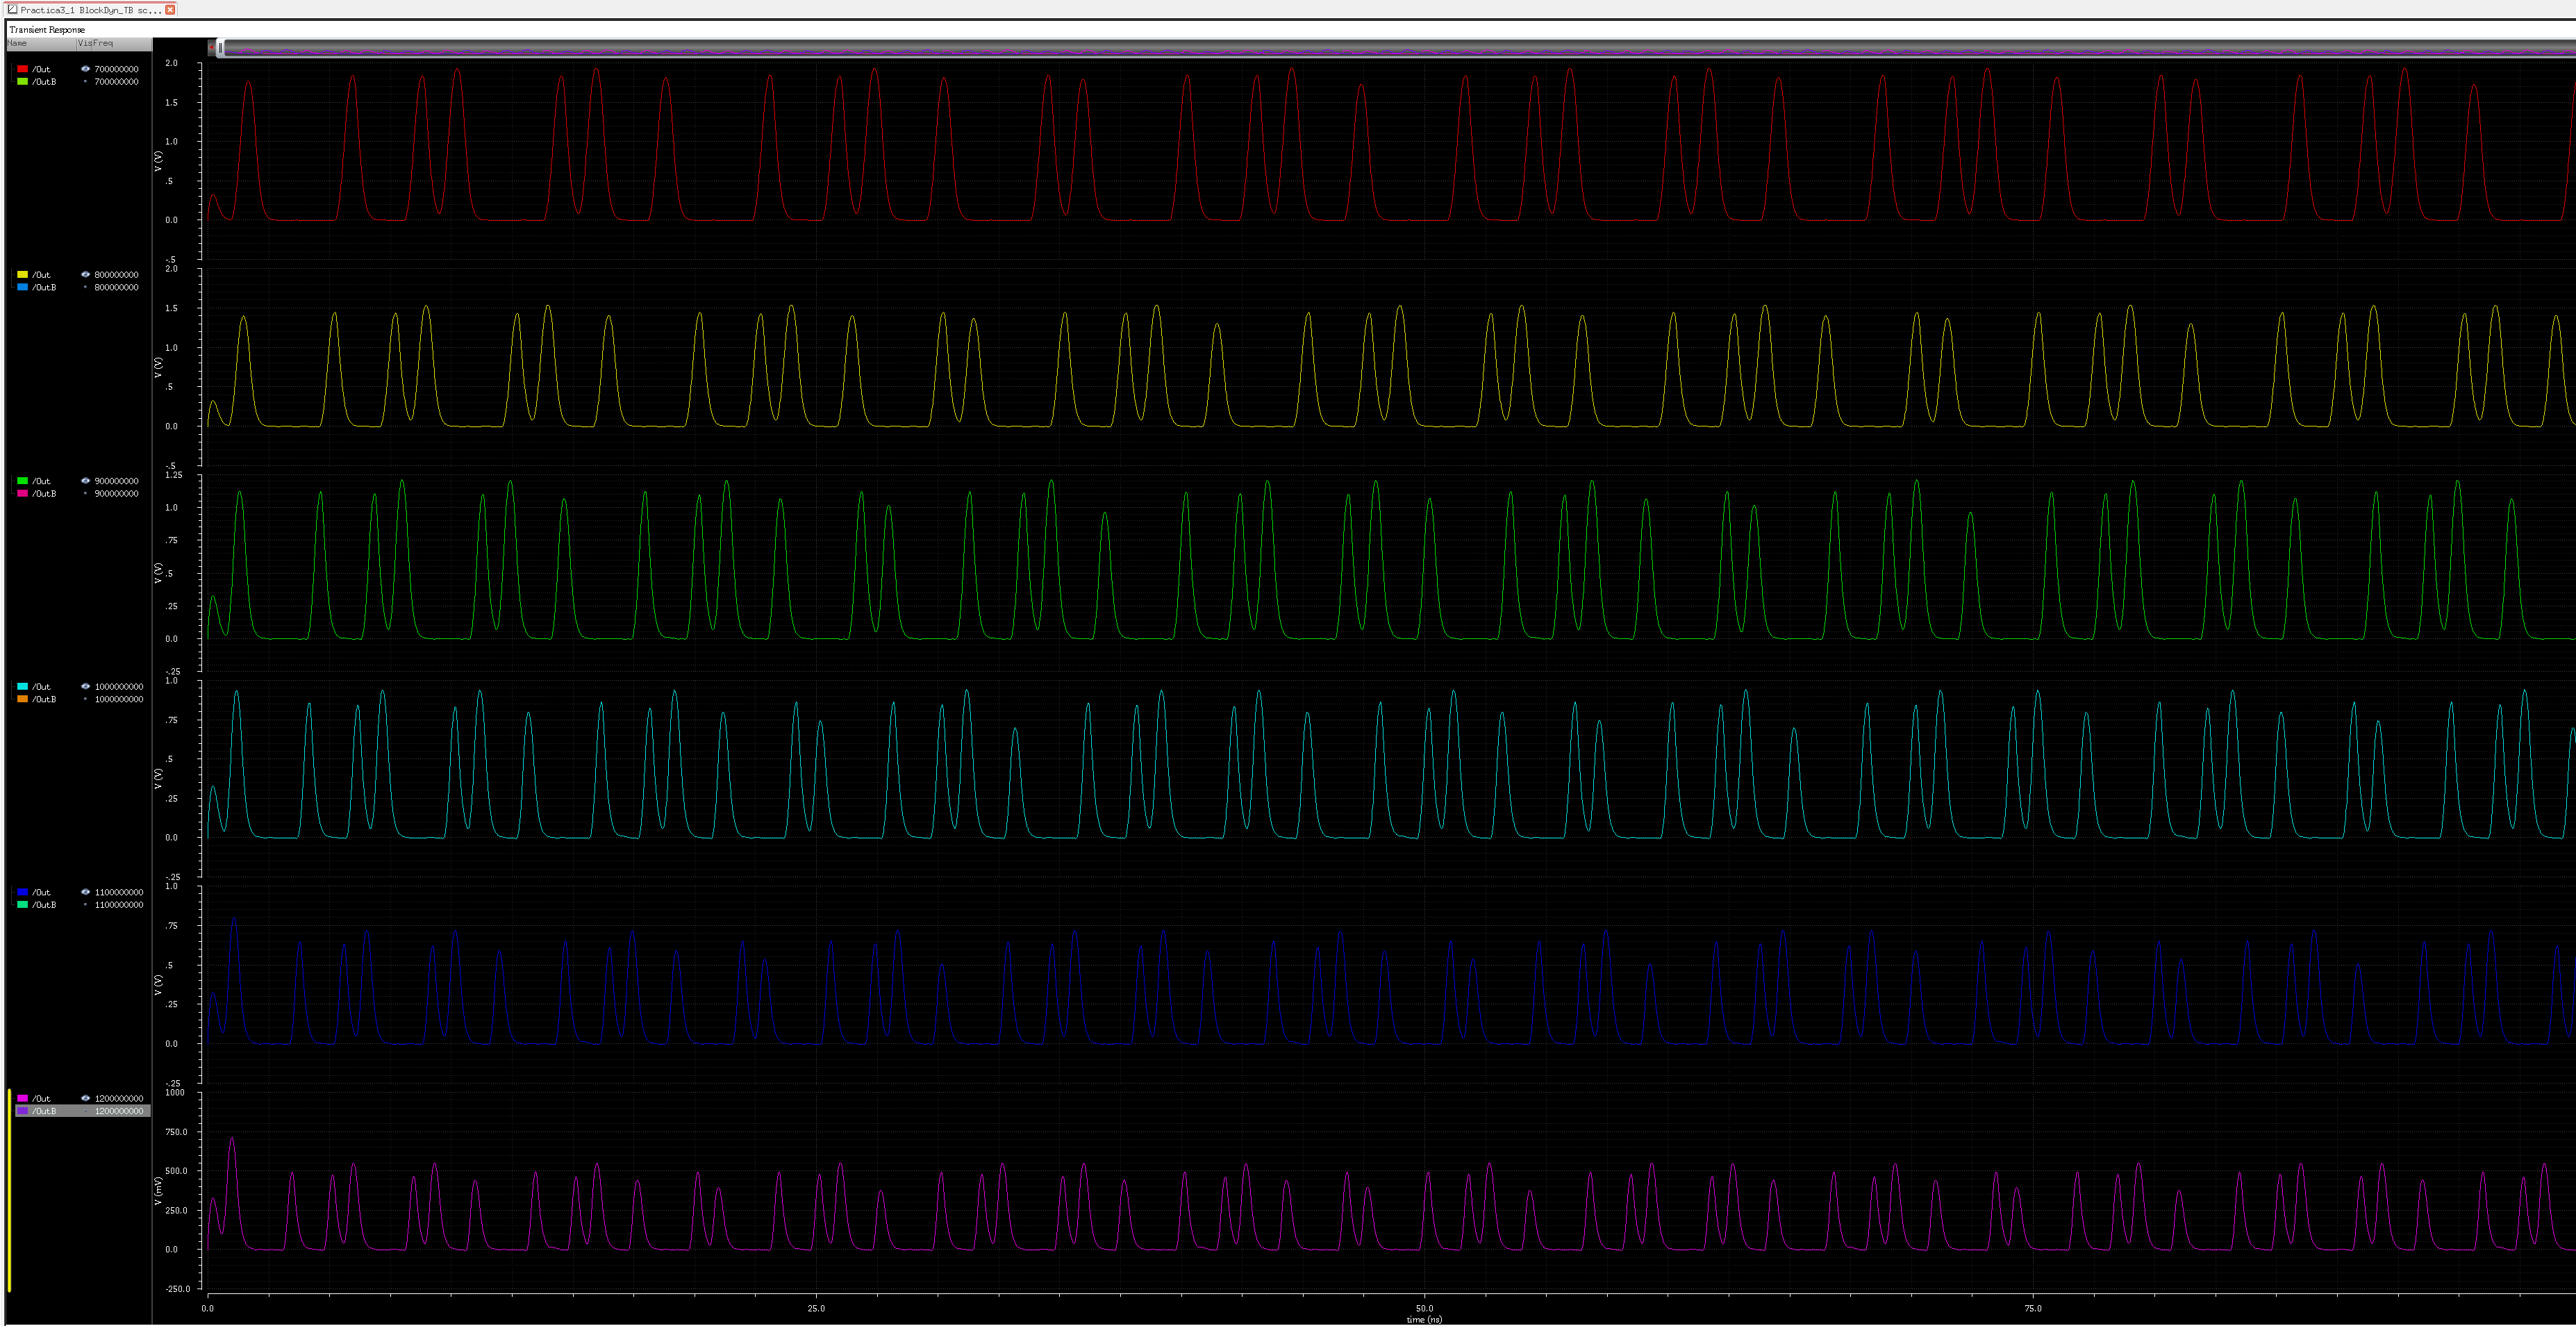
\includegraphics[width=1.1\textwidth]{figures/ParamFreqGraph2.PNG}
\caption{Gráfica del análisis paramétrico 700-1200MHz}
\label{fig:GraphFreq2}
\end {center}
\end{figure} 
Sólamente se muestra la salida Out para mayor claridad. Se puede observar que a medida que aumenta la frecuencia, el nivel de la salida se va reduciendo. Esto se debe a que como cada vez se le da menos tiempo a la evaluación, el nivel de la salida no le da tiempo a subir a un 1 cuando tiene que hacerlo desde el nivel bajo que supone la precarga en este caso. Alrededor de los 700MHz la señal ya llega sólo a la mitad de $V_{DD}$.

\newpage Pero, ¿qué pasaría si se realizara la simulación con un reloj asimétrico dedicándole más tiempo a la precarga o a la evaluación? Bien, estos fueron los resultados:
\begin{figure}[H]%[!ht]
\hspace{-10mm}
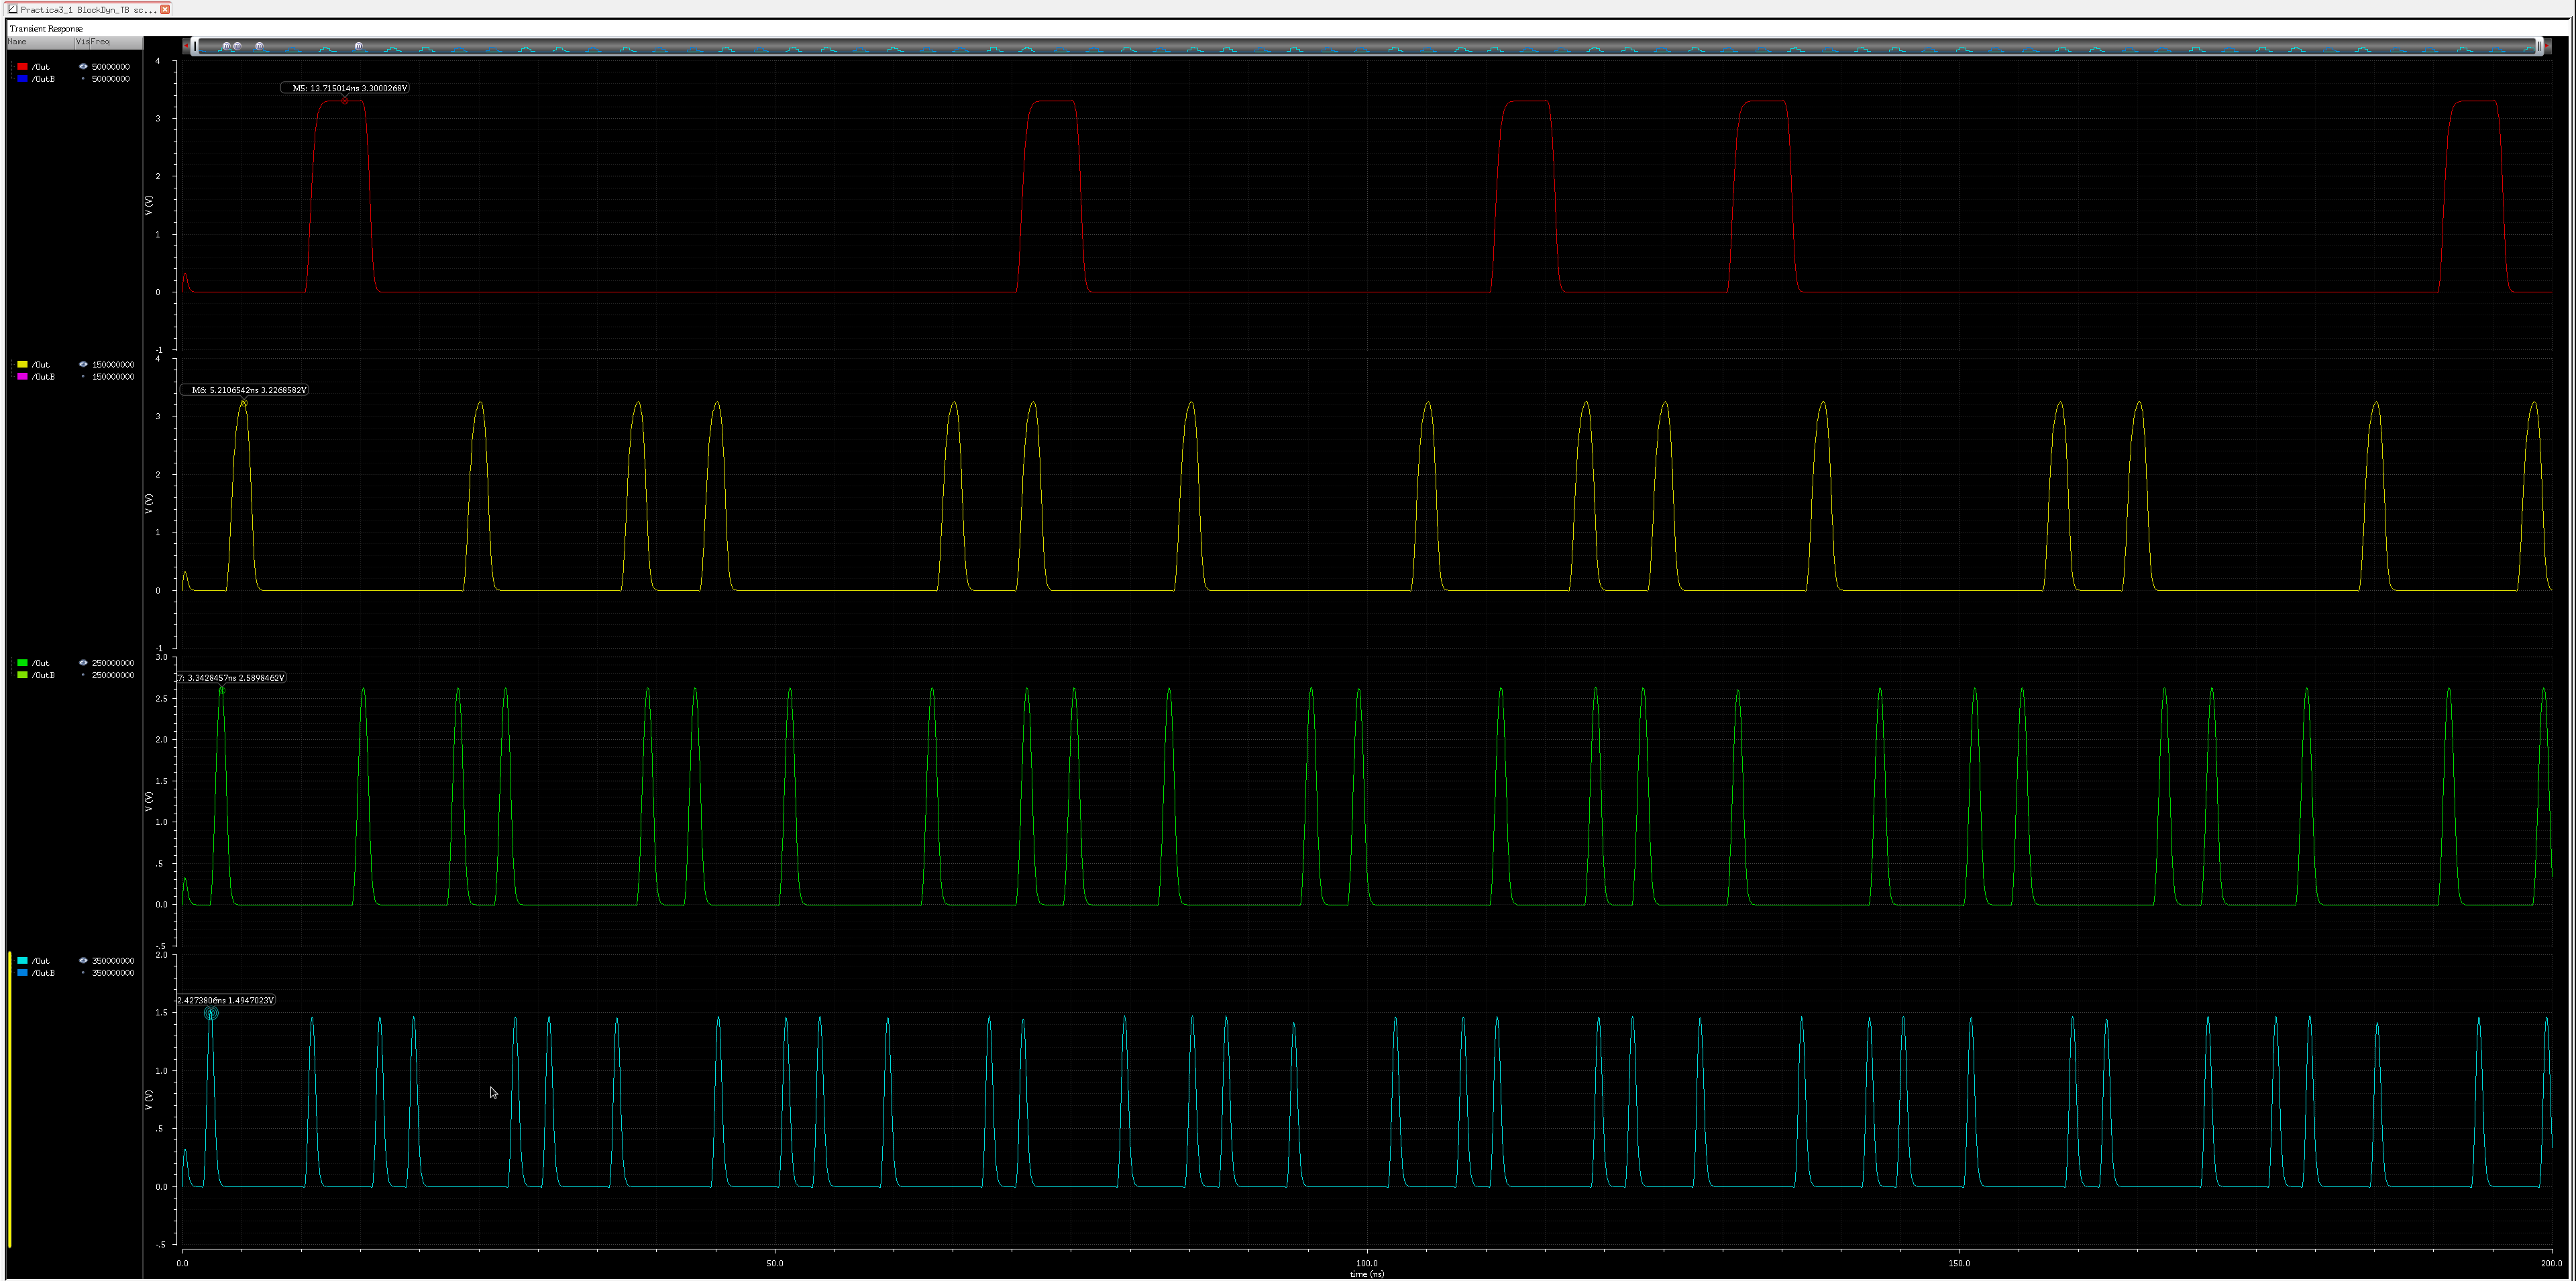
\includegraphics[width=1.2\textwidth]{figures/AsimMuchPreload.png}
\caption{Gráfica del análisis paramétrico 50-350MHz con un 75\% del reloj dedicado a la precarga}
\label{fig:FreqAsimPreload}
\end{figure}
\vspace{-8mm}
\begin{figure}[H]%[!ht]
\hspace{-10mm}
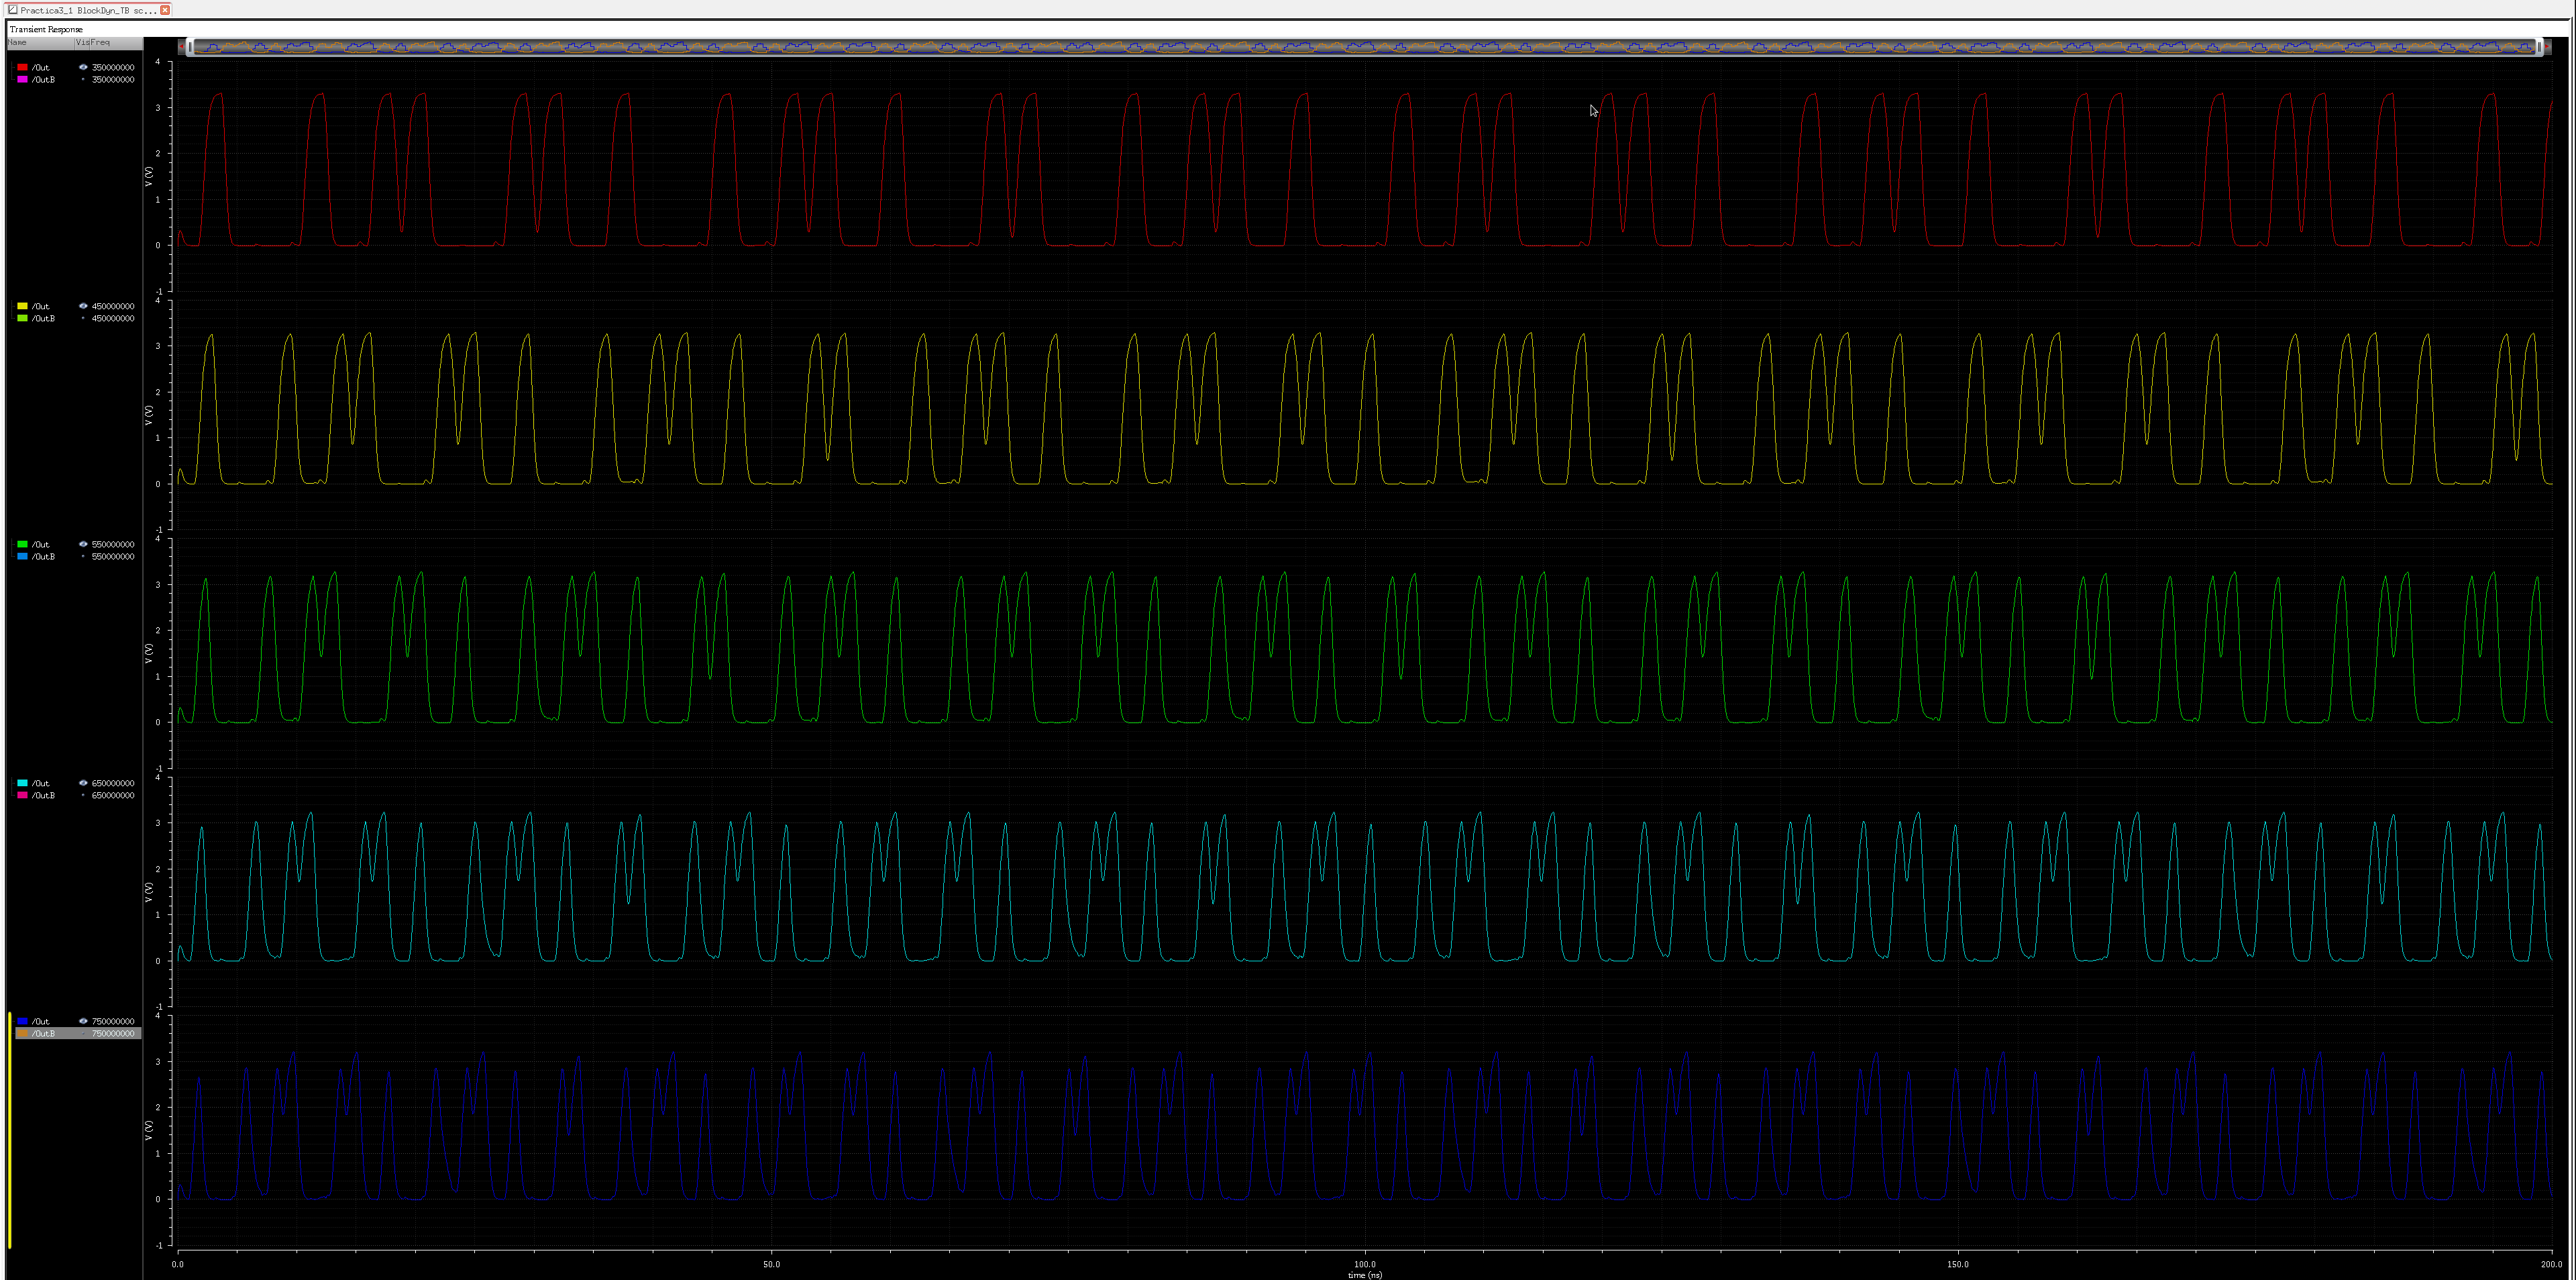
\includegraphics[width=1.2\textwidth]{figures/AsimMuchEval.png}
\caption{Gráfica del análisis paramétrico 350-750MHz con un 75\% del reloj dedicado a la evaluación}
\label{fig:FreqAsimEval}
\end{figure} 
Como se esperaba, la anchura de los pulsos aumenta cuando más porcentaje se le dedique a la evaluación. Además, el nivel de tensión es capaz de llegar los 3.3V a mayor frecuencia que si se le dedicara mayor porcentaje a la precarga. Sin embargo, hay solapamiento de niveles altos de señal a altas frecuencias en la figura \ref{fig:FreqAsimEval} debido a que la precarga dura demasiado poco como para ponerse la salida nivel bajo.
\subsection{Análisis paramétrico con la anchura $W_E$}
Como último paso en esta sección, se simularon para 500MHz de frecuencia, una simulación paramétrica sobre $W_E$, empleando el state anterior y con la siguiente configuración en \textit{Tools->Parametric Analysis}:
\begin{figure}[h]%[!ht]
\begin{center}
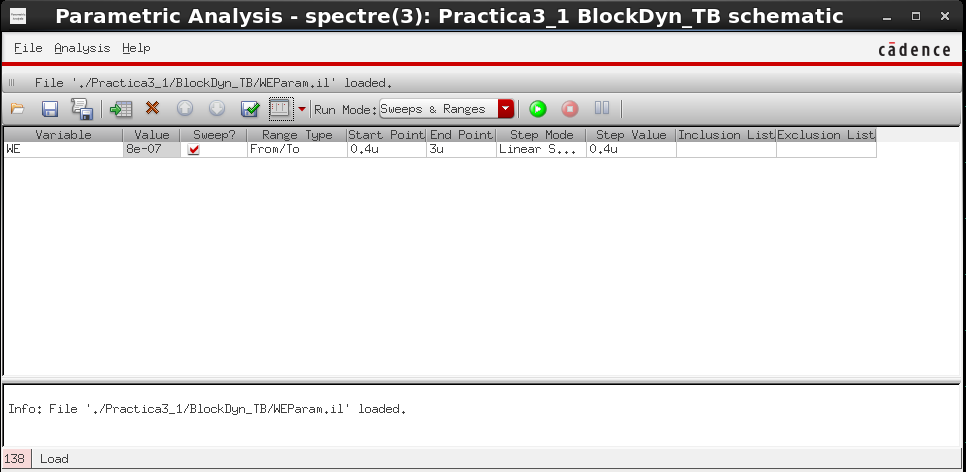
\includegraphics[width=0.8\textwidth]{figures/WEParamConfig.PNG}
\caption{Configuración del análisis paramétrico de $W_E$}
\label{fig:WEConfig}
\end{center}
\end{figure} \newline
Al correr la simulación, se obtuvo esta representación:
\begin{figure}[h]%[!ht]
\hspace{-10mm}
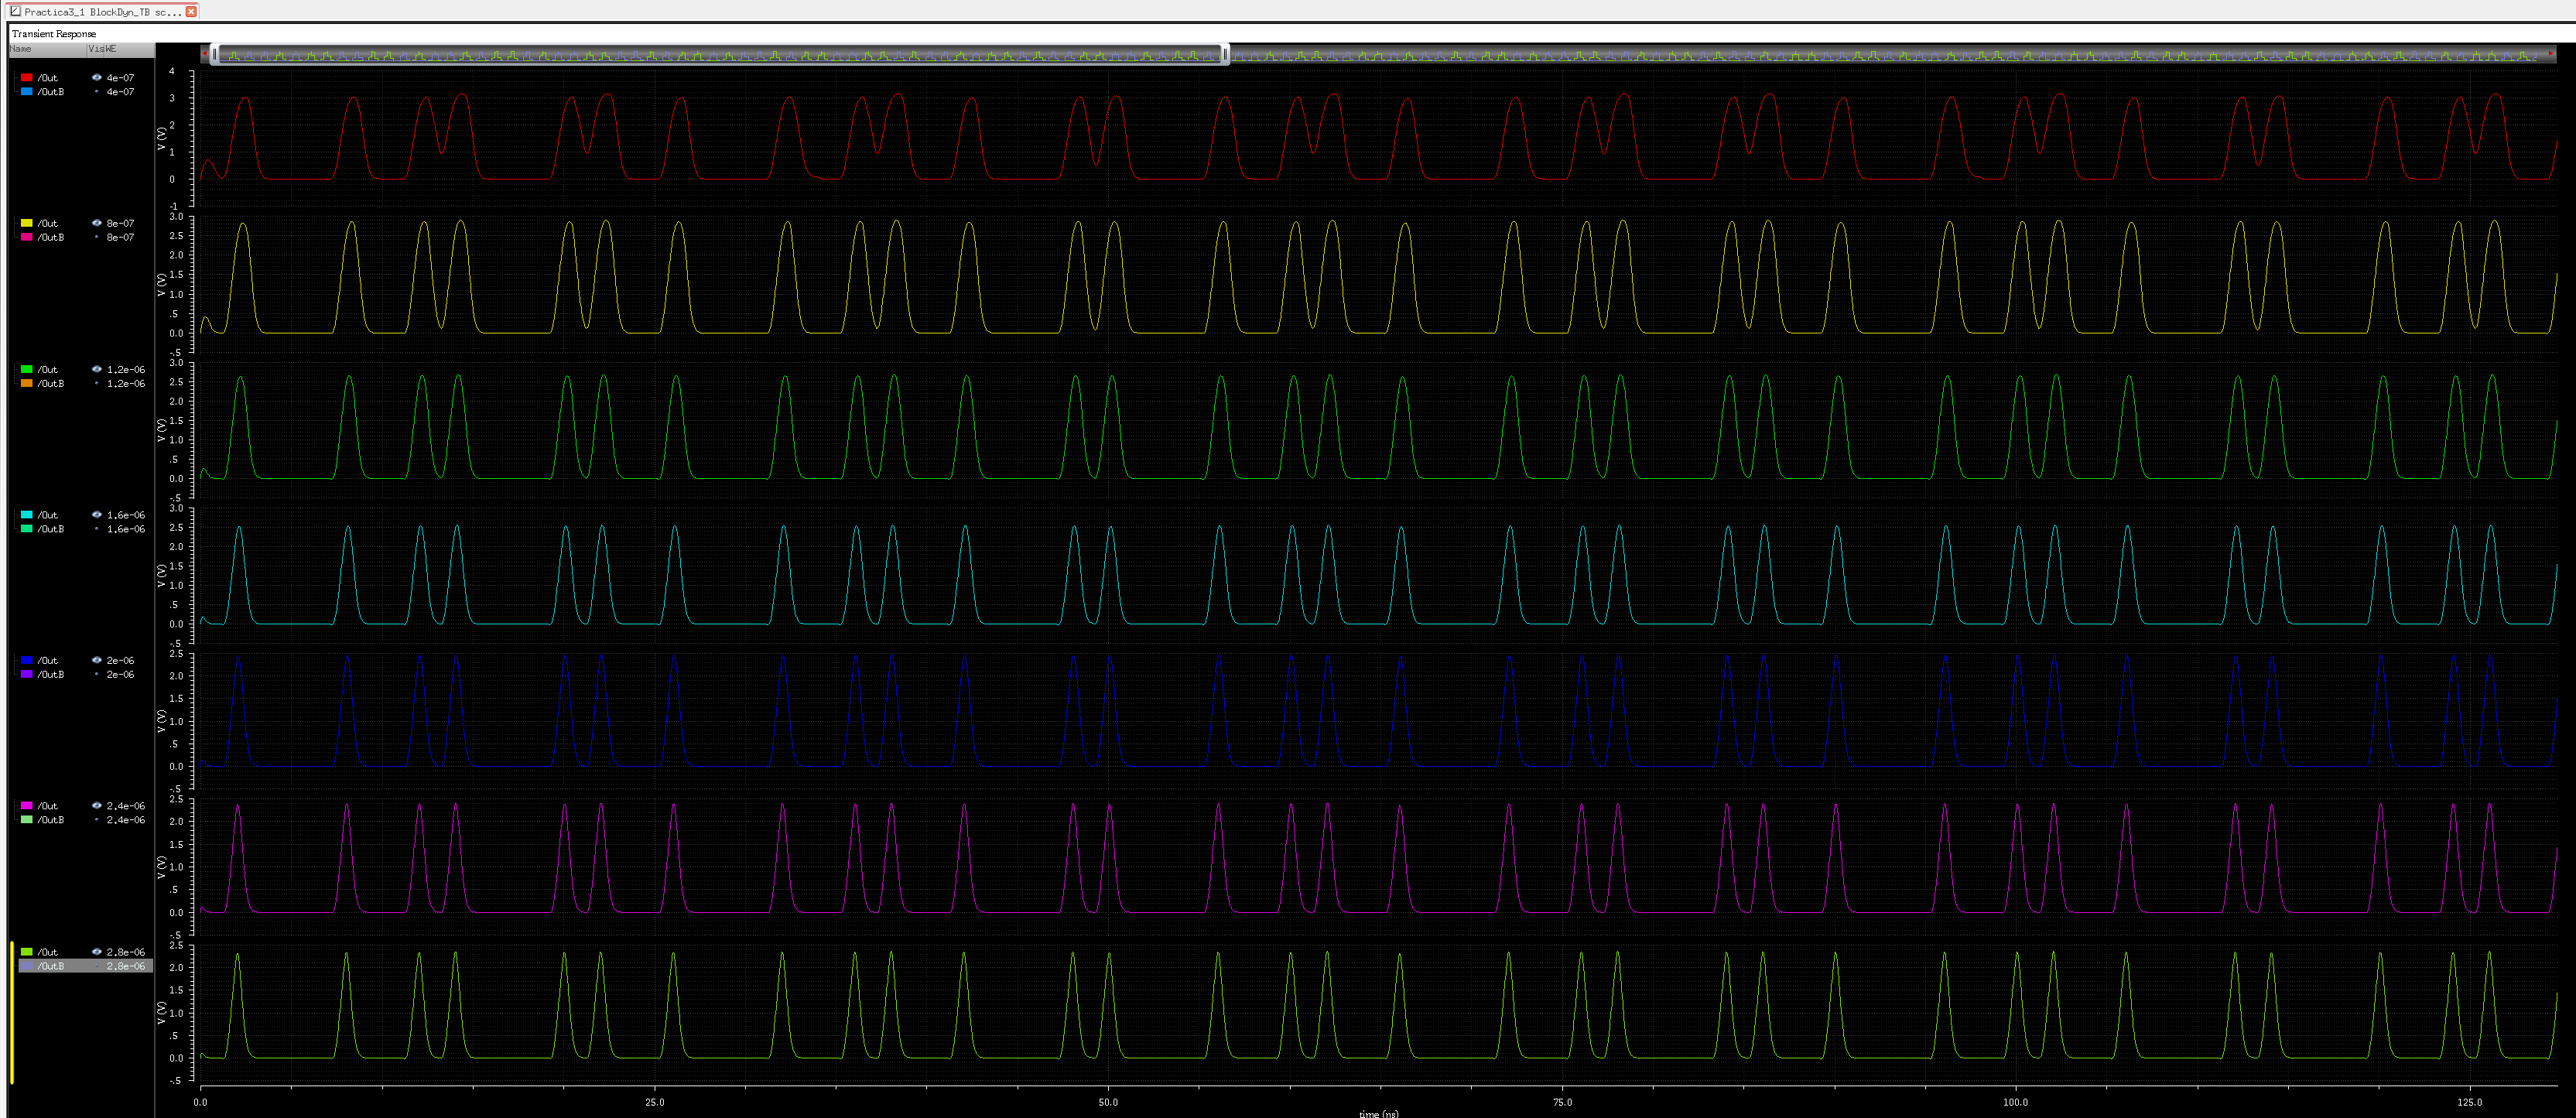
\includegraphics[width=1.2\textwidth]{figures/WEGraph.PNG}
\caption{Gráfica del análisis paramétrico 0.4-3$\mu m$}
\label{fig:WEGraph}
\end{figure} \newline
No se debe aumentar mucho el parámetro $W_E$ ya que ello supone un aumento en el espacio ocupado y mayor carga capacitiva en la línea del reloj, lo que haría que el nivel de la señal se redujera como se ve en los valores más altos de $W_E$ del análisis paramétrico. Por ahora, si se compara con nuestra figura de referencia \ref{fig:GraphState1}, vemos que Out tiene la misma secuencia de valores por lo que la evaluación de momento, está bien con la salvedad del nivel de tensión a la salida ya comentado anteriormente.
\newpage Al igual que con el análisis en frecuencia, se cambió el reloj simétrico por uno asimétrico y, volviéndose a ejecutar la simulación, estos fueron los resultados:
\begin{figure}[H]%[!ht]
\hspace{-10mm}
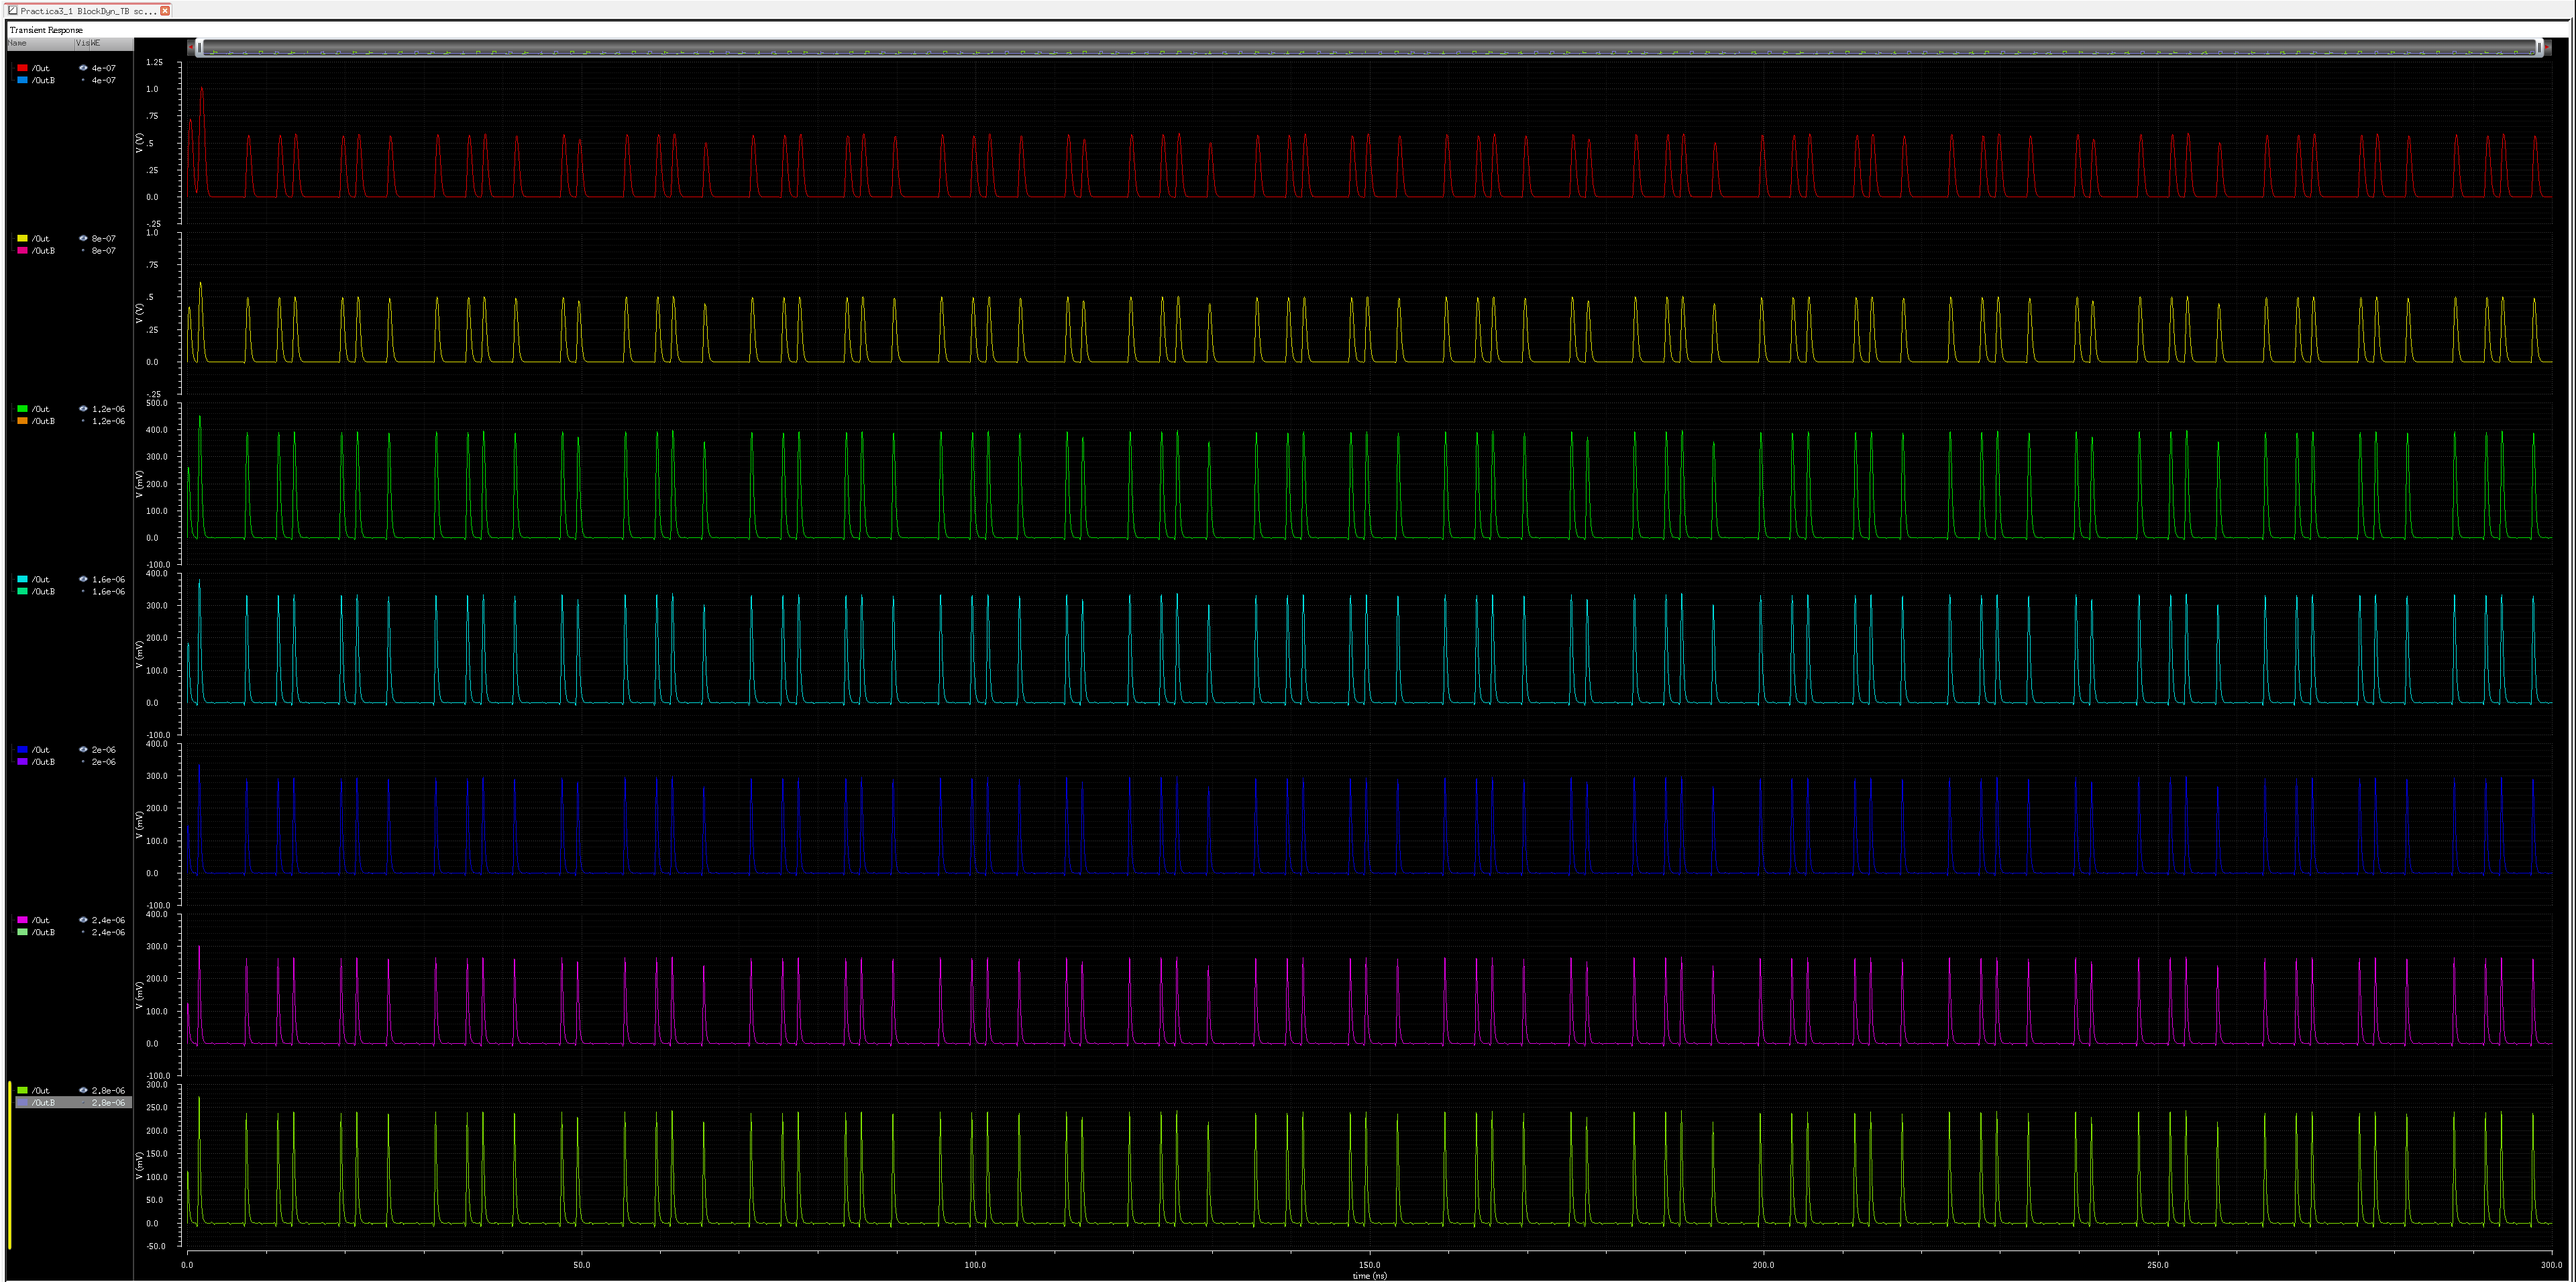
\includegraphics[width=1.2\textwidth]{figures/WEAsimMuchPreload.png}
\caption{Gráfica del análisis paramétrico 0.4-3$\mu m$ con un 75\% del reloj dedicado a la precarga}
\label{fig:WEAsimPreload}
\end{figure}
\vspace{-8mm}
\begin{figure}[H]%[!ht]
\hspace{-10mm}
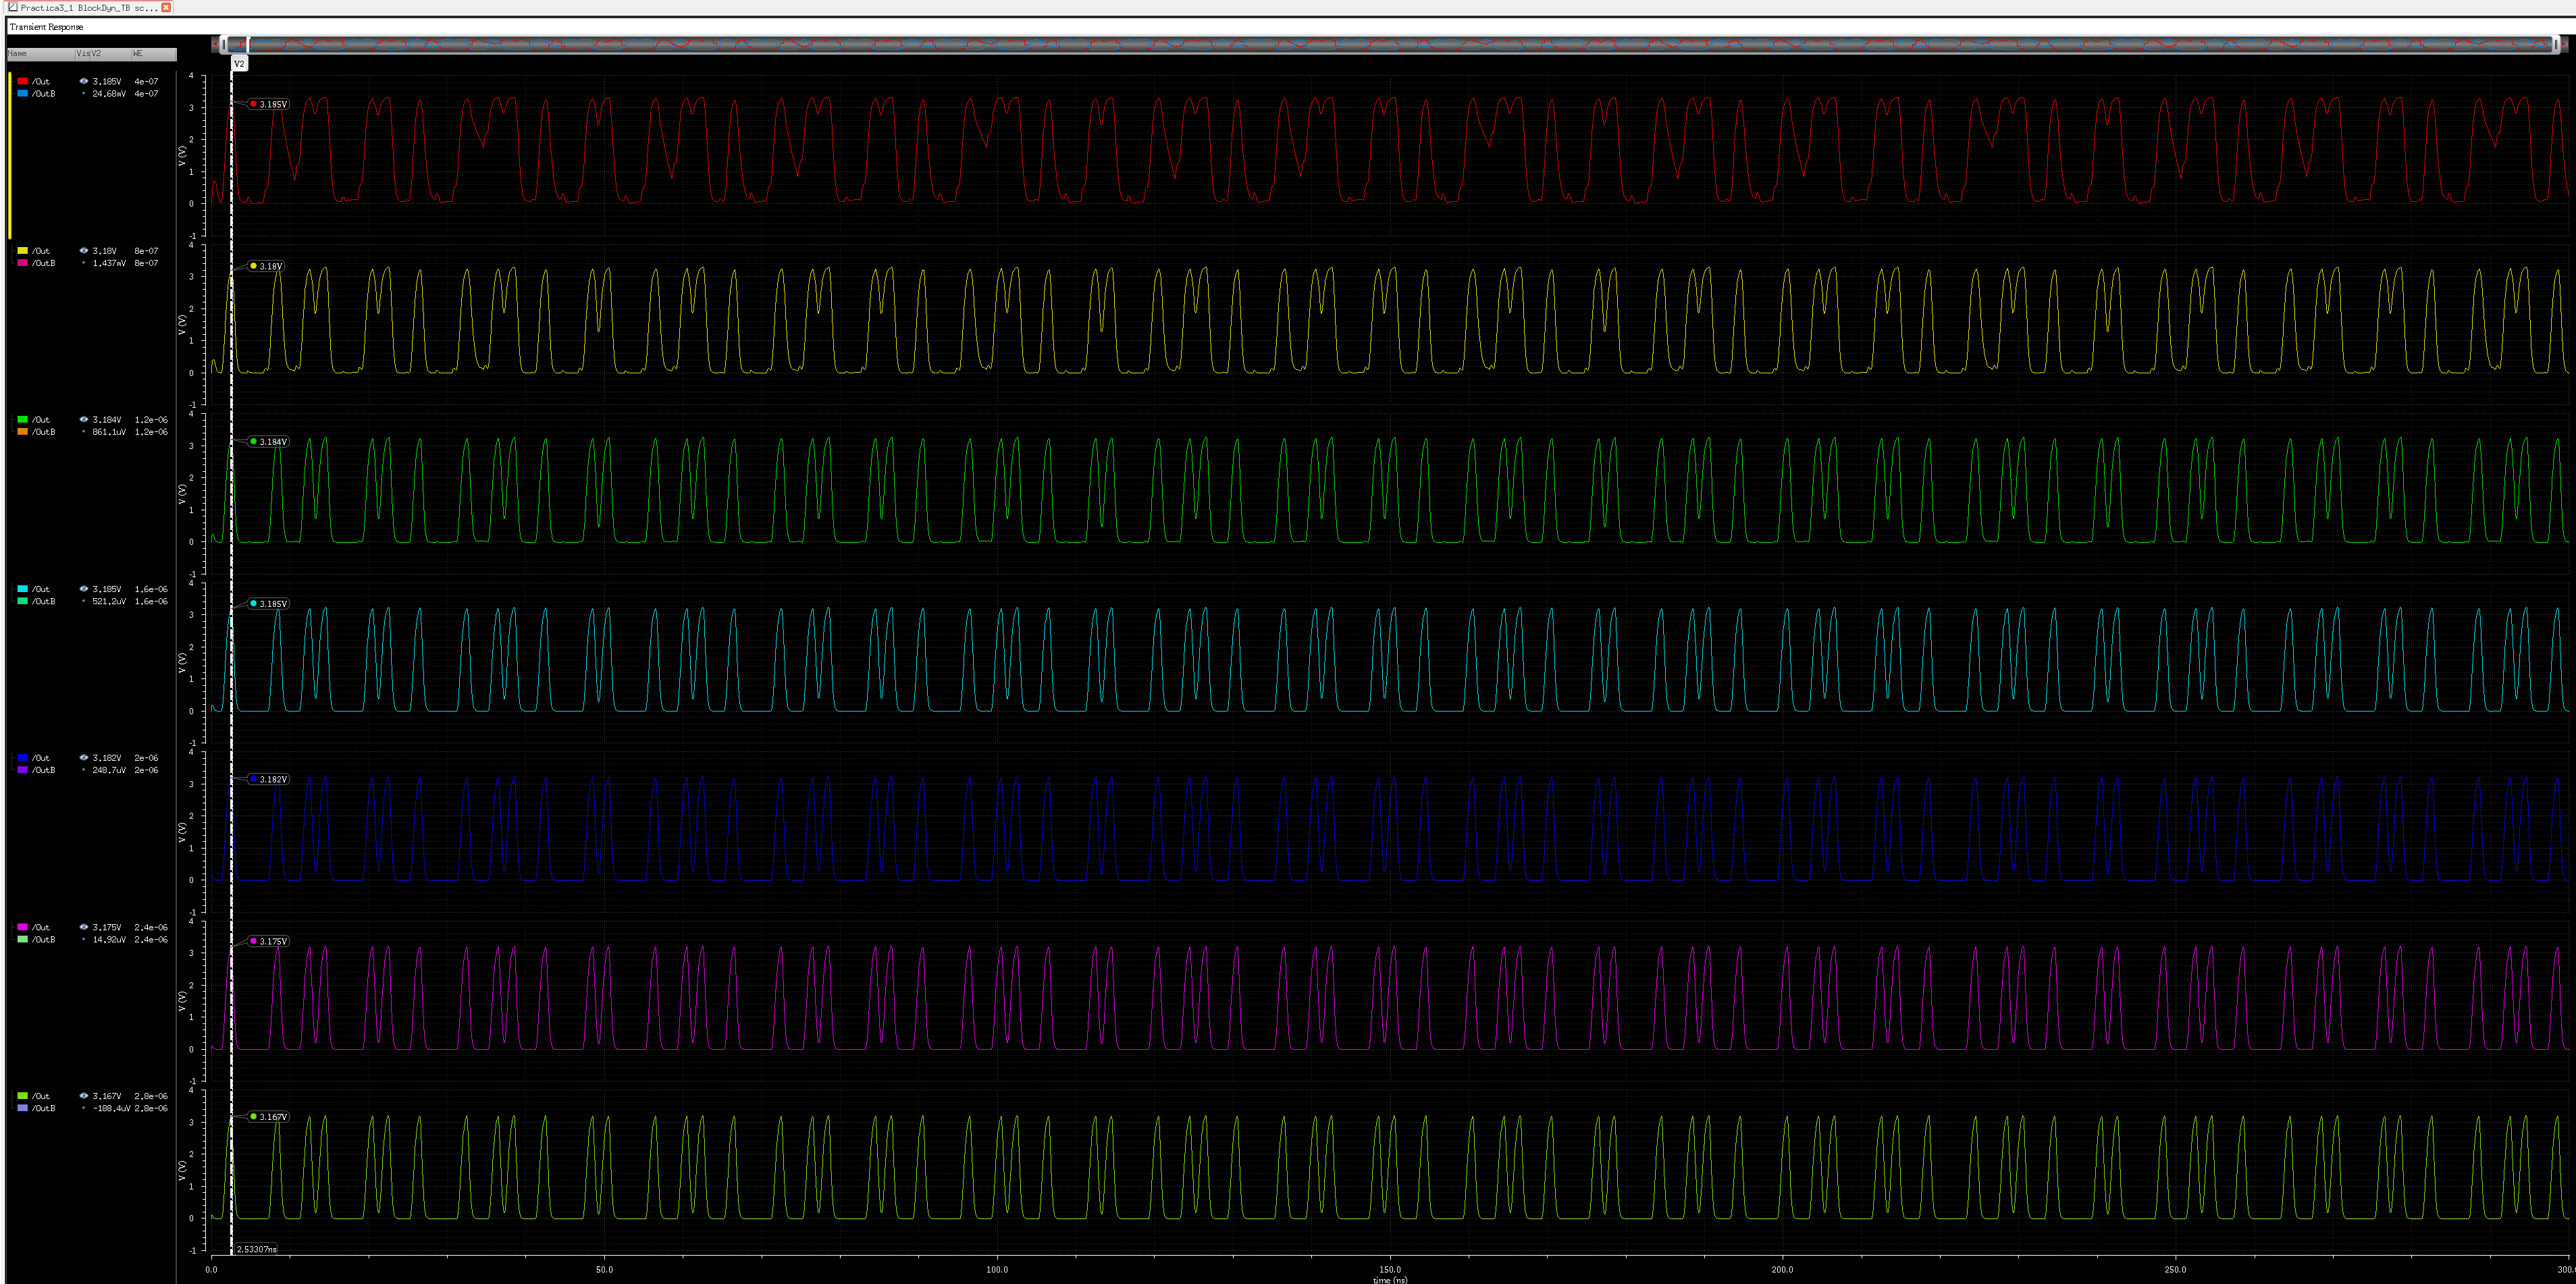
\includegraphics[width=1.2\textwidth]{figures/WEAsimMuchEval.png}
\caption{Gráfica del análisis paramétrico 0.4-3$\mu m$ con un 75\% del reloj dedicado a la evaluación}
\label{fig:WEAsimEval}
\end{figure} 
Si se le dedica demasiado tiempo a la evaluación, la anchura mínima $W_E$ que se debe coger aumenta. Esto se debe a que a mayor $W_E$, mejor evaluación (sin pasarnos mucho con este valor). En caso contrario, debido a que la precarga dura mucho, cuando se debe poner a 1 la salida, esta tiene demasiado poco tiempo para hacerlo y, por tanto no llega a los niveles de tensión requeridos. Habría que coger una $W_E$ más pequeña para disminuir la resistencia y la capacidad de los nMOS y conseguir así alcanzar el valor de tensión de nivel alto.
\restoregeometry